\documentclass[t]{beamer}

% Load general definitions
\input{preamble.tex}

% Specific definitions
\title[]{Algoritmos e Estruturas de Dados III}
\subtitle[]{Tipos de Grafos}
\author[]{Patrícia Lucas\\{\footnotesize }}
\institute{Bacharelado em Sistemas de Informação \\ IFNMG  - Campus Salinas}
\date{\scriptsize Salinas\\Dezembro 2020}

\begin{document}

% cover page
\setbeamertemplate{footline}{}
\begin{frame}

\begin{center}
\includegraphics[width=.15\textwidth]{}
\end{center}
  \titlepage
  \begin{tikzpicture}[remember picture,overlay]
  \node[anchor=south east,xshift=-5pt,yshift=5pt] at (current page.south east) {\tiny Versão 1.2020};
  \node[anchor=south west,yshift=0pt] at (current page.south west) {\includegraphics[width=.25\textwidth]{Logos/salinas_horizontal_jpg.jpg}};
  \end{tikzpicture}  
\end{frame}

% Main slides
\begin{ftst}{Grafo nulo}{Tipos de Grafos}

\begin{itemize}
    \item Um vértice que possui grau zero é um vértice isolado.
    \item É possível que um grafo não contenha nenhuma aresta. 
    \item Nesse caso todos os vértices são isolados e o grafo é chamado grafo nulo.
\end{itemize}
\vone
\centering


\tikzset{every picture/.style={line width=0.75pt}} %set default line width to 0.75pt        

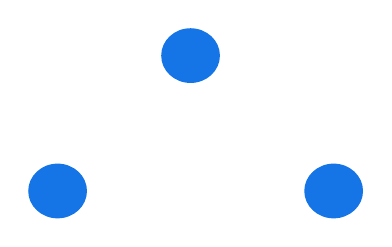
\begin{tikzpicture}[x=0.75pt,y=0.75pt,yscale=-1,xscale=1]
%uncomment if require: \path (0,135); %set diagram left start at 0, and has height of 135

%Shape: Ellipse [id:dp576785563635352] 
\draw  [draw opacity=0][fill={rgb, 255:red, 21; green, 117; blue, 231 }  ,fill opacity=1 ] (88.33,38.19) .. controls (88.33,30.9) and (94.66,25) .. (102.48,25) .. controls (110.29,25) and (116.63,30.9) .. (116.63,38.19) .. controls (116.63,45.47) and (110.29,51.37) .. (102.48,51.37) .. controls (94.66,51.37) and (88.33,45.47) .. (88.33,38.19) -- cycle ;
%Shape: Ellipse [id:dp5059258886052] 
\draw  [draw opacity=0][fill={rgb, 255:red, 21; green, 117; blue, 231 }  ,fill opacity=1 ] (157.27,103.42) .. controls (157.27,96.13) and (163.61,90.23) .. (171.42,90.23) .. controls (179.24,90.23) and (185.58,96.13) .. (185.58,103.42) .. controls (185.58,110.7) and (179.24,116.6) .. (171.42,116.6) .. controls (163.61,116.6) and (157.27,110.7) .. (157.27,103.42) -- cycle ;
%Shape: Ellipse [id:dp140521787960731] 
\draw  [draw opacity=0][fill={rgb, 255:red, 21; green, 117; blue, 231 }  ,fill opacity=1 ] (24.27,103.42) .. controls (24.27,96.13) and (30.61,90.23) .. (38.42,90.23) .. controls (46.24,90.23) and (52.58,96.13) .. (52.58,103.42) .. controls (52.58,110.7) and (46.24,116.6) .. (38.42,116.6) .. controls (30.61,116.6) and (24.27,110.7) .. (24.27,103.42) -- cycle ;




\end{tikzpicture}

\end{ftst}

%=====

\begin{ftst}{Grafo Regular}{Tipos de Grafos}

Um grafo regular é aquele no qual todos os vértices possuem o mesmo grau. Um grafo regular com vértices de grau $k$ é chamado de \textbf{k-regular}.

\vone

\centering 

\tikzset{every picture/.style={line width=0.75pt}} %set default line width to 0.75pt        

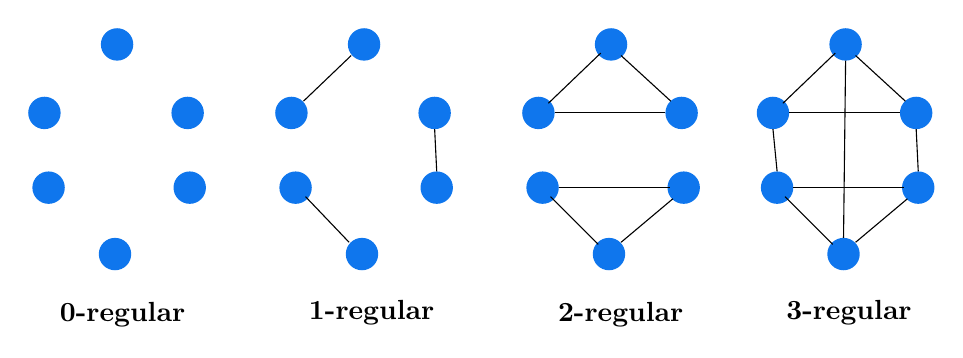
\begin{tikzpicture}[x=0.75pt,y=0.75pt,yscale=-1,xscale=1]
%uncomment if require: \path (0,163); %set diagram left start at 0, and has height of 163

%Shape: Circle [id:dp49108312541965815] 
\draw  [draw opacity=0][fill={rgb, 255:red, 15; green, 118; blue, 237 }  ,fill opacity=1 ] (52,8.81) .. controls (52,4.49) and (55.49,1) .. (59.81,1) .. controls (64.12,1) and (67.61,4.49) .. (67.61,8.81) .. controls (67.61,13.12) and (64.12,16.61) .. (59.81,16.61) .. controls (55.49,16.61) and (52,13.12) .. (52,8.81) -- cycle ;
%Shape: Circle [id:dp4199375150434681] 
\draw  [draw opacity=0][fill={rgb, 255:red, 15; green, 118; blue, 237 }  ,fill opacity=1 ] (87,77.81) .. controls (87,73.49) and (90.49,70) .. (94.81,70) .. controls (99.12,70) and (102.61,73.49) .. (102.61,77.81) .. controls (102.61,82.12) and (99.12,85.61) .. (94.81,85.61) .. controls (90.49,85.61) and (87,82.12) .. (87,77.81) -- cycle ;
%Shape: Circle [id:dp028849324440868296] 
\draw  [draw opacity=0][fill={rgb, 255:red, 15; green, 118; blue, 237 }  ,fill opacity=1 ] (86,41.81) .. controls (86,37.49) and (89.49,34) .. (93.81,34) .. controls (98.12,34) and (101.61,37.49) .. (101.61,41.81) .. controls (101.61,46.12) and (98.12,49.61) .. (93.81,49.61) .. controls (89.49,49.61) and (86,46.12) .. (86,41.81) -- cycle ;
%Shape: Circle [id:dp38070877511653656] 
\draw  [draw opacity=0][fill={rgb, 255:red, 15; green, 118; blue, 237 }  ,fill opacity=1 ] (51,109.81) .. controls (51,105.49) and (54.49,102) .. (58.81,102) .. controls (63.12,102) and (66.61,105.49) .. (66.61,109.81) .. controls (66.61,114.12) and (63.12,117.61) .. (58.81,117.61) .. controls (54.49,117.61) and (51,114.12) .. (51,109.81) -- cycle ;
%Shape: Circle [id:dp03869375459279922] 
\draw  [draw opacity=0][fill={rgb, 255:red, 15; green, 118; blue, 237 }  ,fill opacity=1 ] (19,77.81) .. controls (19,73.49) and (22.49,70) .. (26.81,70) .. controls (31.12,70) and (34.61,73.49) .. (34.61,77.81) .. controls (34.61,82.12) and (31.12,85.61) .. (26.81,85.61) .. controls (22.49,85.61) and (19,82.12) .. (19,77.81) -- cycle ;
%Shape: Circle [id:dp7178304097649642] 
\draw  [draw opacity=0][fill={rgb, 255:red, 15; green, 118; blue, 237 }  ,fill opacity=1 ] (17,41.81) .. controls (17,37.49) and (20.49,34) .. (24.81,34) .. controls (29.12,34) and (32.61,37.49) .. (32.61,41.81) .. controls (32.61,46.12) and (29.12,49.61) .. (24.81,49.61) .. controls (20.49,49.61) and (17,46.12) .. (17,41.81) -- cycle ;
%Shape: Circle [id:dp315593455618312] 
\draw  [draw opacity=0][fill={rgb, 255:red, 15; green, 118; blue, 237 }  ,fill opacity=1 ] (171,8.81) .. controls (171,4.49) and (174.49,1) .. (178.81,1) .. controls (183.12,1) and (186.61,4.49) .. (186.61,8.81) .. controls (186.61,13.12) and (183.12,16.61) .. (178.81,16.61) .. controls (174.49,16.61) and (171,13.12) .. (171,8.81) -- cycle ;
%Shape: Circle [id:dp6898296345502213] 
\draw  [draw opacity=0][fill={rgb, 255:red, 15; green, 118; blue, 237 }  ,fill opacity=1 ] (206,77.81) .. controls (206,73.49) and (209.49,70) .. (213.81,70) .. controls (218.12,70) and (221.61,73.49) .. (221.61,77.81) .. controls (221.61,82.12) and (218.12,85.61) .. (213.81,85.61) .. controls (209.49,85.61) and (206,82.12) .. (206,77.81) -- cycle ;
%Shape: Circle [id:dp4917941827813932] 
\draw  [draw opacity=0][fill={rgb, 255:red, 15; green, 118; blue, 237 }  ,fill opacity=1 ] (205,41.81) .. controls (205,37.49) and (208.49,34) .. (212.81,34) .. controls (217.12,34) and (220.61,37.49) .. (220.61,41.81) .. controls (220.61,46.12) and (217.12,49.61) .. (212.81,49.61) .. controls (208.49,49.61) and (205,46.12) .. (205,41.81) -- cycle ;
%Shape: Circle [id:dp3327375167586579] 
\draw  [draw opacity=0][fill={rgb, 255:red, 15; green, 118; blue, 237 }  ,fill opacity=1 ] (170,109.81) .. controls (170,105.49) and (173.49,102) .. (177.81,102) .. controls (182.12,102) and (185.61,105.49) .. (185.61,109.81) .. controls (185.61,114.12) and (182.12,117.61) .. (177.81,117.61) .. controls (173.49,117.61) and (170,114.12) .. (170,109.81) -- cycle ;
%Shape: Circle [id:dp8245825748303128] 
\draw  [draw opacity=0][fill={rgb, 255:red, 15; green, 118; blue, 237 }  ,fill opacity=1 ] (138,77.81) .. controls (138,73.49) and (141.49,70) .. (145.81,70) .. controls (150.12,70) and (153.61,73.49) .. (153.61,77.81) .. controls (153.61,82.12) and (150.12,85.61) .. (145.81,85.61) .. controls (141.49,85.61) and (138,82.12) .. (138,77.81) -- cycle ;
%Shape: Circle [id:dp12115223390362106] 
\draw  [draw opacity=0][fill={rgb, 255:red, 15; green, 118; blue, 237 }  ,fill opacity=1 ] (136,41.81) .. controls (136,37.49) and (139.49,34) .. (143.81,34) .. controls (148.12,34) and (151.61,37.49) .. (151.61,41.81) .. controls (151.61,46.12) and (148.12,49.61) .. (143.81,49.61) .. controls (139.49,49.61) and (136,46.12) .. (136,41.81) -- cycle ;
%Shape: Circle [id:dp17987039516237124] 
\draw  [draw opacity=0][fill={rgb, 255:red, 15; green, 118; blue, 237 }  ,fill opacity=1 ] (290,8.81) .. controls (290,4.49) and (293.49,1) .. (297.81,1) .. controls (302.12,1) and (305.61,4.49) .. (305.61,8.81) .. controls (305.61,13.12) and (302.12,16.61) .. (297.81,16.61) .. controls (293.49,16.61) and (290,13.12) .. (290,8.81) -- cycle ;
%Shape: Circle [id:dp22777952380488076] 
\draw  [draw opacity=0][fill={rgb, 255:red, 15; green, 118; blue, 237 }  ,fill opacity=1 ] (325,77.81) .. controls (325,73.49) and (328.49,70) .. (332.81,70) .. controls (337.12,70) and (340.61,73.49) .. (340.61,77.81) .. controls (340.61,82.12) and (337.12,85.61) .. (332.81,85.61) .. controls (328.49,85.61) and (325,82.12) .. (325,77.81) -- cycle ;
%Shape: Circle [id:dp8927240300940578] 
\draw  [draw opacity=0][fill={rgb, 255:red, 15; green, 118; blue, 237 }  ,fill opacity=1 ] (324,41.81) .. controls (324,37.49) and (327.49,34) .. (331.81,34) .. controls (336.12,34) and (339.61,37.49) .. (339.61,41.81) .. controls (339.61,46.12) and (336.12,49.61) .. (331.81,49.61) .. controls (327.49,49.61) and (324,46.12) .. (324,41.81) -- cycle ;
%Shape: Circle [id:dp7069135206955519] 
\draw  [draw opacity=0][fill={rgb, 255:red, 15; green, 118; blue, 237 }  ,fill opacity=1 ] (289,109.81) .. controls (289,105.49) and (292.49,102) .. (296.81,102) .. controls (301.12,102) and (304.61,105.49) .. (304.61,109.81) .. controls (304.61,114.12) and (301.12,117.61) .. (296.81,117.61) .. controls (292.49,117.61) and (289,114.12) .. (289,109.81) -- cycle ;
%Shape: Circle [id:dp6478424024118168] 
\draw  [draw opacity=0][fill={rgb, 255:red, 15; green, 118; blue, 237 }  ,fill opacity=1 ] (257,77.81) .. controls (257,73.49) and (260.49,70) .. (264.81,70) .. controls (269.12,70) and (272.61,73.49) .. (272.61,77.81) .. controls (272.61,82.12) and (269.12,85.61) .. (264.81,85.61) .. controls (260.49,85.61) and (257,82.12) .. (257,77.81) -- cycle ;
%Shape: Circle [id:dp6117436353734191] 
\draw  [draw opacity=0][fill={rgb, 255:red, 15; green, 118; blue, 237 }  ,fill opacity=1 ] (255,41.81) .. controls (255,37.49) and (258.49,34) .. (262.81,34) .. controls (267.12,34) and (270.61,37.49) .. (270.61,41.81) .. controls (270.61,46.12) and (267.12,49.61) .. (262.81,49.61) .. controls (258.49,49.61) and (255,46.12) .. (255,41.81) -- cycle ;
%Straight Lines [id:da9490530906867032] 
\draw    (149.61,36.15) -- (172.61,14.15) ;
%Straight Lines [id:da6747299259400299] 
\draw    (213.81,70) -- (212.81,49.61) ;
%Straight Lines [id:da09167271201940697] 
\draw    (150.61,82.15) -- (171.61,104.15) ;
%Straight Lines [id:da7283359050643692] 
\draw    (267.61,37.15) -- (292.81,13) ;
%Straight Lines [id:da16762476067874577] 
\draw    (326.61,36.15) -- (302.61,14.15) ;
%Straight Lines [id:da32277945205702485] 
\draw    (270.61,41.81) -- (324,41.81) ;
%Straight Lines [id:da35163301408420433] 
\draw    (272.61,77.81) -- (326,77.81) ;
%Straight Lines [id:da6533402296072959] 
\draw    (268.61,82.15) -- (291.61,105.15) ;
%Straight Lines [id:da4178653695385772] 
\draw    (302.61,104.15) -- (327.61,83.15) ;
%Shape: Circle [id:dp2685686616579994] 
\draw  [draw opacity=0][fill={rgb, 255:red, 15; green, 118; blue, 237 }  ,fill opacity=1 ] (403,8.81) .. controls (403,4.49) and (406.49,1) .. (410.81,1) .. controls (415.12,1) and (418.61,4.49) .. (418.61,8.81) .. controls (418.61,13.12) and (415.12,16.61) .. (410.81,16.61) .. controls (406.49,16.61) and (403,13.12) .. (403,8.81) -- cycle ;
%Shape: Circle [id:dp44699968893161435] 
\draw  [draw opacity=0][fill={rgb, 255:red, 15; green, 118; blue, 237 }  ,fill opacity=1 ] (438,77.81) .. controls (438,73.49) and (441.49,70) .. (445.81,70) .. controls (450.12,70) and (453.61,73.49) .. (453.61,77.81) .. controls (453.61,82.12) and (450.12,85.61) .. (445.81,85.61) .. controls (441.49,85.61) and (438,82.12) .. (438,77.81) -- cycle ;
%Shape: Circle [id:dp3608775636168653] 
\draw  [draw opacity=0][fill={rgb, 255:red, 15; green, 118; blue, 237 }  ,fill opacity=1 ] (437,41.81) .. controls (437,37.49) and (440.49,34) .. (444.81,34) .. controls (449.12,34) and (452.61,37.49) .. (452.61,41.81) .. controls (452.61,46.12) and (449.12,49.61) .. (444.81,49.61) .. controls (440.49,49.61) and (437,46.12) .. (437,41.81) -- cycle ;
%Shape: Circle [id:dp6658595225184782] 
\draw  [draw opacity=0][fill={rgb, 255:red, 15; green, 118; blue, 237 }  ,fill opacity=1 ] (402,109.81) .. controls (402,105.49) and (405.49,102) .. (409.81,102) .. controls (414.12,102) and (417.61,105.49) .. (417.61,109.81) .. controls (417.61,114.12) and (414.12,117.61) .. (409.81,117.61) .. controls (405.49,117.61) and (402,114.12) .. (402,109.81) -- cycle ;
%Shape: Circle [id:dp7900754494287732] 
\draw  [draw opacity=0][fill={rgb, 255:red, 15; green, 118; blue, 237 }  ,fill opacity=1 ] (370,77.81) .. controls (370,73.49) and (373.49,70) .. (377.81,70) .. controls (382.12,70) and (385.61,73.49) .. (385.61,77.81) .. controls (385.61,82.12) and (382.12,85.61) .. (377.81,85.61) .. controls (373.49,85.61) and (370,82.12) .. (370,77.81) -- cycle ;
%Shape: Circle [id:dp7714892205399768] 
\draw  [draw opacity=0][fill={rgb, 255:red, 15; green, 118; blue, 237 }  ,fill opacity=1 ] (368,41.81) .. controls (368,37.49) and (371.49,34) .. (375.81,34) .. controls (380.12,34) and (383.61,37.49) .. (383.61,41.81) .. controls (383.61,46.12) and (380.12,49.61) .. (375.81,49.61) .. controls (371.49,49.61) and (368,46.12) .. (368,41.81) -- cycle ;
%Straight Lines [id:da33628682504934426] 
\draw    (380.61,37.15) -- (405.81,13) ;
%Straight Lines [id:da17674633798335537] 
\draw    (439.61,36.15) -- (415.61,14.15) ;
%Straight Lines [id:da036056929302281215] 
\draw    (383.61,41.81) -- (437,41.81) ;
%Straight Lines [id:da33006375305403046] 
\draw    (385.61,77.81) -- (439,77.81) ;
%Straight Lines [id:da4652546841512679] 
\draw    (381.61,82.15) -- (404.61,105.15) ;
%Straight Lines [id:da9158558589705772] 
\draw    (415.61,104.15) -- (440.61,83.15) ;
%Straight Lines [id:da3034333168018355] 
\draw    (410.81,16.61) -- (409.81,102) ;
%Straight Lines [id:da37479007720261337] 
\draw    (375.81,49.61) -- (377.81,70) ;
%Straight Lines [id:da8769841070714419] 
\draw    (444.81,49.61) -- (445.81,70) ;

% Text Node
\draw (31,132) node [anchor=north west][inner sep=0.75pt]   [align=left] {\textbf{0-regular}};
% Text Node
\draw (151,130.97) node [anchor=north west][inner sep=0.75pt]   [align=left] {\textbf{1-regular}};
% Text Node
\draw (271,131.97) node [anchor=north west][inner sep=0.75pt]   [align=left] {\textbf{2-regular}};
% Text Node
\draw (381,130.97) node [anchor=north west][inner sep=0.75pt]   [align=left] {\textbf{3-regular}};


\end{tikzpicture}

\end{ftst}

%=====

\begin{ftst}{Grafo Completo}{Tipos de Grafos}

Um grafo com $n$ vértices é chamado de completo, e denotado de $K_n$ , se para cada par de vértices distintos existe exatamente uma aresta conectando-os. Ou seja, é um grafo simples que contém o número máximo de arestas.
\vone
\centering
\includegraphics[scale=0.4]{Figuras/grafo_completo.jpg}


\end{ftst}

%=====

\begin{ftst}{Grafo Completo}{Tipos de Grafos}

O número de arestas em um grafo completo é: 
\vone
\centering
\huge
$|E| = |V| (|V| - 1) / 2$


\end{ftst}

%=====

\begin{ftst}{Complemento de um Grafo}{Tipos de Grafos}
\justifying
O Complemento de um grafo simples $G$, denotado por $G'$, é o grafo simples que possui o mesmo conjunto de vértices de $G$, e tal que dois vértices distintos são adjacentes em $G'$ se não são em $G$.
\vone
\vone
\centering


\tikzset{every picture/.style={line width=0.75pt}} %set default line width to 0.75pt        

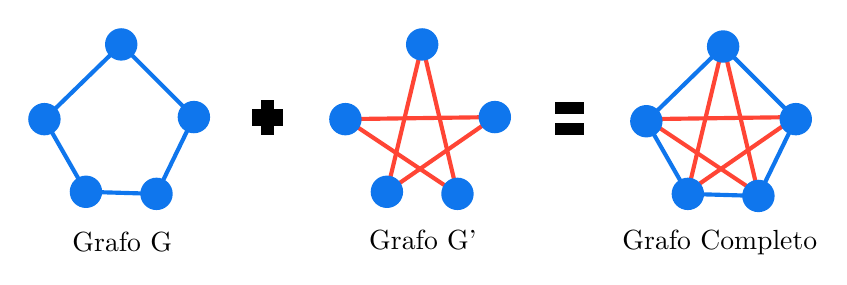
\begin{tikzpicture}[x=0.75pt,y=0.75pt,yscale=-1,xscale=1]
%uncomment if require: \path (0,146); %set diagram left start at 0, and has height of 146

%Straight Lines [id:da6286716115891509] 
\draw [color={rgb, 255:red, 255; green, 69; blue, 53 }  ,draw opacity=1 ][line width=1.5]    (388.81,99.81) -- (371.81,27.81) ;
%Straight Lines [id:da8615097224096446] 
\draw [color={rgb, 255:red, 255; green, 69; blue, 53 }  ,draw opacity=1 ][line width=1.5]    (406.81,62.81) -- (334.81,63.81) ;
%Straight Lines [id:da6874816210575747] 
\draw [color={rgb, 255:red, 255; green, 69; blue, 53 }  ,draw opacity=1 ][line width=1.5]    (388.81,99.81) -- (334.81,63.81) ;
%Straight Lines [id:da7467287538393712] 
\draw [color={rgb, 255:red, 255; green, 69; blue, 53 }  ,draw opacity=1 ][line width=1.5]    (354.81,98.81) -- (406.81,62.81) ;
%Straight Lines [id:da22709598157536104] 
\draw [color={rgb, 255:red, 255; green, 69; blue, 53 }  ,draw opacity=1 ][line width=1.5]    (371.81,27.81) -- (354.81,98.81) ;
%Straight Lines [id:da8128576904560505] 
\draw [color={rgb, 255:red, 255; green, 69; blue, 53 }  ,draw opacity=1 ][line width=1.5]    (243.81,99.81) -- (226.81,27.81) ;
%Straight Lines [id:da46056102558920564] 
\draw [color={rgb, 255:red, 255; green, 69; blue, 53 }  ,draw opacity=1 ][line width=1.5]    (261.81,62.81) -- (189.81,63.81) ;
%Straight Lines [id:da5780673278719084] 
\draw [color={rgb, 255:red, 255; green, 69; blue, 53 }  ,draw opacity=1 ][line width=1.5]    (243.81,99.81) -- (189.81,63.81) ;
%Straight Lines [id:da10083150854017786] 
\draw [color={rgb, 255:red, 255; green, 69; blue, 53 }  ,draw opacity=1 ][line width=1.5]    (209.81,98.81) -- (261.81,62.81) ;
%Straight Lines [id:da39379403255252776] 
\draw [color={rgb, 255:red, 255; green, 69; blue, 53 }  ,draw opacity=1 ][line width=1.5]    (226.81,27.81) -- (209.81,98.81) ;
%Shape: Circle [id:dp17206767364522735] 
\draw  [draw opacity=0][fill={rgb, 255:red, 15; green, 118; blue, 237 }  ,fill opacity=1 ] (74,27.81) .. controls (74,23.49) and (77.49,20) .. (81.81,20) .. controls (86.12,20) and (89.61,23.49) .. (89.61,27.81) .. controls (89.61,32.12) and (86.12,35.61) .. (81.81,35.61) .. controls (77.49,35.61) and (74,32.12) .. (74,27.81) -- cycle ;
%Shape: Circle [id:dp8817745518555591] 
\draw  [draw opacity=0][fill={rgb, 255:red, 15; green, 118; blue, 237 }  ,fill opacity=1 ] (91,99.81) .. controls (91,95.49) and (94.49,92) .. (98.81,92) .. controls (103.12,92) and (106.61,95.49) .. (106.61,99.81) .. controls (106.61,104.12) and (103.12,107.61) .. (98.81,107.61) .. controls (94.49,107.61) and (91,104.12) .. (91,99.81) -- cycle ;
%Shape: Circle [id:dp983446861828384] 
\draw  [draw opacity=0][fill={rgb, 255:red, 15; green, 118; blue, 237 }  ,fill opacity=1 ] (109,62.81) .. controls (109,58.49) and (112.49,55) .. (116.81,55) .. controls (121.12,55) and (124.61,58.49) .. (124.61,62.81) .. controls (124.61,67.12) and (121.12,70.61) .. (116.81,70.61) .. controls (112.49,70.61) and (109,67.12) .. (109,62.81) -- cycle ;
%Shape: Circle [id:dp3733314601313251] 
\draw  [draw opacity=0][fill={rgb, 255:red, 15; green, 118; blue, 237 }  ,fill opacity=1 ] (57,98.81) .. controls (57,94.49) and (60.49,91) .. (64.81,91) .. controls (69.12,91) and (72.61,94.49) .. (72.61,98.81) .. controls (72.61,103.12) and (69.12,106.61) .. (64.81,106.61) .. controls (60.49,106.61) and (57,103.12) .. (57,98.81) -- cycle ;
%Shape: Circle [id:dp31508397542449407] 
\draw  [draw opacity=0][fill={rgb, 255:red, 15; green, 118; blue, 237 }  ,fill opacity=1 ] (37,63.81) .. controls (37,59.49) and (40.49,56) .. (44.81,56) .. controls (49.12,56) and (52.61,59.49) .. (52.61,63.81) .. controls (52.61,68.12) and (49.12,71.61) .. (44.81,71.61) .. controls (40.49,71.61) and (37,68.12) .. (37,63.81) -- cycle ;
%Straight Lines [id:da4019504678384127] 
\draw [color={rgb, 255:red, 15; green, 118; blue, 237 }  ,draw opacity=1 ][line width=1.5]    (44.81,63.81) -- (81.81,27.81) ;
%Straight Lines [id:da33751766037536557] 
\draw [color={rgb, 255:red, 15; green, 118; blue, 237 }  ,draw opacity=1 ][line width=1.5]    (116.81,62.81) -- (81.81,27.81) ;
%Straight Lines [id:da36837524239373765] 
\draw [color={rgb, 255:red, 15; green, 118; blue, 237 }  ,draw opacity=1 ][line width=1.5]    (64.81,98.81) -- (44.81,63.81) ;
%Straight Lines [id:da5684634535440216] 
\draw [color={rgb, 255:red, 15; green, 118; blue, 237 }  ,draw opacity=1 ][line width=1.5]    (98.81,99.81) -- (116.81,62.81) ;
%Straight Lines [id:da7336404196898463] 
\draw [color={rgb, 255:red, 15; green, 118; blue, 237 }  ,draw opacity=1 ][line width=1.5]    (64.81,98.81) -- (98.81,99.81) ;
%Shape: Circle [id:dp2133071752077793] 
\draw  [draw opacity=0][fill={rgb, 255:red, 15; green, 118; blue, 237 }  ,fill opacity=1 ] (219,27.81) .. controls (219,23.49) and (222.49,20) .. (226.81,20) .. controls (231.12,20) and (234.61,23.49) .. (234.61,27.81) .. controls (234.61,32.12) and (231.12,35.61) .. (226.81,35.61) .. controls (222.49,35.61) and (219,32.12) .. (219,27.81) -- cycle ;
%Shape: Circle [id:dp7970171128213852] 
\draw  [draw opacity=0][fill={rgb, 255:red, 15; green, 118; blue, 237 }  ,fill opacity=1 ] (236,99.81) .. controls (236,95.49) and (239.49,92) .. (243.81,92) .. controls (248.12,92) and (251.61,95.49) .. (251.61,99.81) .. controls (251.61,104.12) and (248.12,107.61) .. (243.81,107.61) .. controls (239.49,107.61) and (236,104.12) .. (236,99.81) -- cycle ;
%Shape: Circle [id:dp8772839428999042] 
\draw  [draw opacity=0][fill={rgb, 255:red, 15; green, 118; blue, 237 }  ,fill opacity=1 ] (254,62.81) .. controls (254,58.49) and (257.49,55) .. (261.81,55) .. controls (266.12,55) and (269.61,58.49) .. (269.61,62.81) .. controls (269.61,67.12) and (266.12,70.61) .. (261.81,70.61) .. controls (257.49,70.61) and (254,67.12) .. (254,62.81) -- cycle ;
%Shape: Circle [id:dp08146825073335462] 
\draw  [draw opacity=0][fill={rgb, 255:red, 15; green, 118; blue, 237 }  ,fill opacity=1 ] (202,98.81) .. controls (202,94.49) and (205.49,91) .. (209.81,91) .. controls (214.12,91) and (217.61,94.49) .. (217.61,98.81) .. controls (217.61,103.12) and (214.12,106.61) .. (209.81,106.61) .. controls (205.49,106.61) and (202,103.12) .. (202,98.81) -- cycle ;
%Shape: Circle [id:dp2604299443287845] 
\draw  [draw opacity=0][fill={rgb, 255:red, 15; green, 118; blue, 237 }  ,fill opacity=1 ] (182,63.81) .. controls (182,59.49) and (185.49,56) .. (189.81,56) .. controls (194.12,56) and (197.61,59.49) .. (197.61,63.81) .. controls (197.61,68.12) and (194.12,71.61) .. (189.81,71.61) .. controls (185.49,71.61) and (182,68.12) .. (182,63.81) -- cycle ;
%Shape: Circle [id:dp02208476926602243] 
\draw  [draw opacity=0][fill={rgb, 255:red, 15; green, 118; blue, 237 }  ,fill opacity=1 ] (364,28.81) .. controls (364,24.49) and (367.49,21) .. (371.81,21) .. controls (376.12,21) and (379.61,24.49) .. (379.61,28.81) .. controls (379.61,33.12) and (376.12,36.61) .. (371.81,36.61) .. controls (367.49,36.61) and (364,33.12) .. (364,28.81) -- cycle ;
%Shape: Circle [id:dp14745587301806817] 
\draw  [draw opacity=0][fill={rgb, 255:red, 15; green, 118; blue, 237 }  ,fill opacity=1 ] (381,100.81) .. controls (381,96.49) and (384.49,93) .. (388.81,93) .. controls (393.12,93) and (396.61,96.49) .. (396.61,100.81) .. controls (396.61,105.12) and (393.12,108.61) .. (388.81,108.61) .. controls (384.49,108.61) and (381,105.12) .. (381,100.81) -- cycle ;
%Shape: Circle [id:dp03821434537628687] 
\draw  [draw opacity=0][fill={rgb, 255:red, 15; green, 118; blue, 237 }  ,fill opacity=1 ] (399,63.81) .. controls (399,59.49) and (402.49,56) .. (406.81,56) .. controls (411.12,56) and (414.61,59.49) .. (414.61,63.81) .. controls (414.61,68.12) and (411.12,71.61) .. (406.81,71.61) .. controls (402.49,71.61) and (399,68.12) .. (399,63.81) -- cycle ;
%Shape: Circle [id:dp14052332172014892] 
\draw  [draw opacity=0][fill={rgb, 255:red, 15; green, 118; blue, 237 }  ,fill opacity=1 ] (347,99.81) .. controls (347,95.49) and (350.49,92) .. (354.81,92) .. controls (359.12,92) and (362.61,95.49) .. (362.61,99.81) .. controls (362.61,104.12) and (359.12,107.61) .. (354.81,107.61) .. controls (350.49,107.61) and (347,104.12) .. (347,99.81) -- cycle ;
%Shape: Circle [id:dp08749177881137715] 
\draw  [draw opacity=0][fill={rgb, 255:red, 15; green, 118; blue, 237 }  ,fill opacity=1 ] (327,64.81) .. controls (327,60.49) and (330.49,57) .. (334.81,57) .. controls (339.12,57) and (342.61,60.49) .. (342.61,64.81) .. controls (342.61,69.12) and (339.12,72.61) .. (334.81,72.61) .. controls (330.49,72.61) and (327,69.12) .. (327,64.81) -- cycle ;
%Straight Lines [id:da0162842505226648] 
\draw [color={rgb, 255:red, 15; green, 118; blue, 237 }  ,draw opacity=1 ][line width=1.5]    (334.81,64.81) -- (371.81,28.81) ;
%Straight Lines [id:da5332427745678958] 
\draw [color={rgb, 255:red, 15; green, 118; blue, 237 }  ,draw opacity=1 ][line width=1.5]    (406.81,63.81) -- (371.81,28.81) ;
%Straight Lines [id:da906855391597275] 
\draw [color={rgb, 255:red, 15; green, 118; blue, 237 }  ,draw opacity=1 ][line width=1.5]    (354.81,99.81) -- (334.81,64.81) ;
%Straight Lines [id:da09115093571142174] 
\draw [color={rgb, 255:red, 15; green, 118; blue, 237 }  ,draw opacity=1 ][line width=1.5]    (388.81,100.81) -- (406.81,63.81) ;
%Straight Lines [id:da591316390817122] 
\draw [color={rgb, 255:red, 15; green, 118; blue, 237 }  ,draw opacity=1 ][line width=1.5]    (354.81,99.81) -- (388.81,100.81) ;
%Shape: Cross [id:dp6301285378327248] 
\draw  [fill={rgb, 255:red, 0; green, 0; blue, 0 }  ,fill opacity=1 ] (149.38,55.01) -- (155.22,55.01) -- (155.22,59.39) -- (159.61,59.39) -- (159.61,66.62) -- (155.22,66.62) -- (155.22,71) -- (149.38,71) -- (149.38,66.62) -- (145,66.62) -- (145,59.39) -- (149.38,59.39) -- cycle ;
%Shape: Rectangle [id:dp5532971331016707] 
\draw  [fill={rgb, 255:red, 0; green, 0; blue, 0 }  ,fill opacity=1 ] (291,56) -- (304.61,56) -- (304.61,61.01) -- (291,61.01) -- cycle ;
%Shape: Rectangle [id:dp852512220039451] 
\draw  [fill={rgb, 255:red, 0; green, 0; blue, 0 }  ,fill opacity=1 ] (291,66) -- (304.61,66) -- (304.61,71.01) -- (291,71.01) -- cycle ;

% Text Node
\draw (57,117) node [anchor=north west][inner sep=0.75pt]   [align=left] {Grafo G};
% Text Node
\draw (200,115.97) node [anchor=north west][inner sep=0.75pt]   [align=left] {Grafo G'};
% Text Node
\draw (322,115.97) node [anchor=north west][inner sep=0.75pt]   [align=left] {Grafo Completo};


\end{tikzpicture}\\

\end{ftst}

%=====

\begin{ftst}{Subgrafos}{Tipos de Grafos}

Um subgrafo $G'$ do grafo $G = (V,E)$ é um grafo $(V',E')$ tal que $V' \subseteq V$ e $E' \subseteq E$.                    

\begin{itemize}
    \item Todo grafo é subgrafo dele mesmo.
    \item O subgrafo de um subgrafo de $G$ é um subgrafo de $G$.
    \item Um vértice de $G$ é um subgrafo de $G$.
\end{itemize}
\vone
\centering


\tikzset{every picture/.style={line width=0.75pt}} %set default line width to 0.75pt        

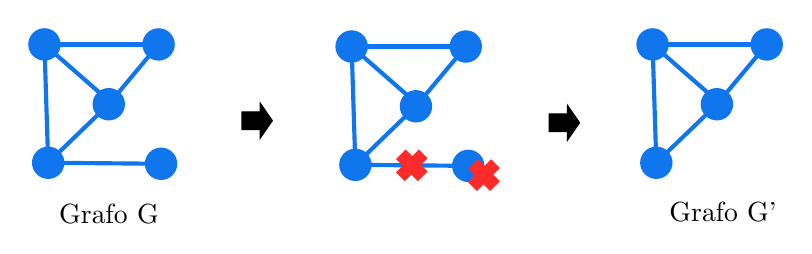
\begin{tikzpicture}[x=0.75pt,y=0.75pt,yscale=-1,xscale=1]
%uncomment if require: \path (0,131); %set diagram left start at 0, and has height of 131

%Shape: Circle [id:dp792626211844353] 
\draw  [draw opacity=0][fill={rgb, 255:red, 15; green, 118; blue, 237 }  ,fill opacity=1 ] (77,29.81) .. controls (77,25.49) and (80.49,22) .. (84.81,22) .. controls (89.12,22) and (92.61,25.49) .. (92.61,29.81) .. controls (92.61,34.12) and (89.12,37.61) .. (84.81,37.61) .. controls (80.49,37.61) and (77,34.12) .. (77,29.81) -- cycle ;
%Shape: Circle [id:dp8214150916748093] 
\draw  [draw opacity=0][fill={rgb, 255:red, 15; green, 118; blue, 237 }  ,fill opacity=1 ] (78.19,87.31) .. controls (78.19,82.99) and (81.69,79.5) .. (86,79.5) .. controls (90.31,79.5) and (93.81,82.99) .. (93.81,87.31) .. controls (93.81,91.62) and (90.31,95.11) .. (86,95.11) .. controls (81.69,95.11) and (78.19,91.62) .. (78.19,87.31) -- cycle ;
%Shape: Circle [id:dp35149982634567056] 
\draw  [draw opacity=0][fill={rgb, 255:red, 15; green, 118; blue, 237 }  ,fill opacity=1 ] (53,58.61) .. controls (53,54.3) and (56.49,50.81) .. (60.81,50.81) .. controls (65.12,50.81) and (68.61,54.3) .. (68.61,58.61) .. controls (68.61,62.92) and (65.12,66.42) .. (60.81,66.42) .. controls (56.49,66.42) and (53,62.92) .. (53,58.61) -- cycle ;
%Shape: Circle [id:dp32845900936445527] 
\draw  [draw opacity=0][fill={rgb, 255:red, 15; green, 118; blue, 237 }  ,fill opacity=1 ] (23.81,86.81) .. controls (23.81,82.49) and (27.3,79) .. (31.61,79) .. controls (35.92,79) and (39.42,82.49) .. (39.42,86.81) .. controls (39.42,91.12) and (35.92,94.61) .. (31.61,94.61) .. controls (27.3,94.61) and (23.81,91.12) .. (23.81,86.81) -- cycle ;
%Shape: Circle [id:dp7223842986862556] 
\draw  [draw opacity=0][fill={rgb, 255:red, 15; green, 118; blue, 237 }  ,fill opacity=1 ] (22,29.81) .. controls (22,25.49) and (25.49,22) .. (29.81,22) .. controls (34.12,22) and (37.61,25.49) .. (37.61,29.81) .. controls (37.61,34.12) and (34.12,37.61) .. (29.81,37.61) .. controls (25.49,37.61) and (22,34.12) .. (22,29.81) -- cycle ;
%Straight Lines [id:da7272749351487289] 
\draw [color={rgb, 255:red, 15; green, 118; blue, 237 }  ,draw opacity=1 ][line width=1.5]    (31.61,86.81) -- (29.81,29.81) ;
%Straight Lines [id:da18029477303082908] 
\draw [color={rgb, 255:red, 15; green, 118; blue, 237 }  ,draw opacity=1 ][line width=1.5]    (84.81,29.81) -- (29.81,29.81) ;
%Straight Lines [id:da24696977957569044] 
\draw [color={rgb, 255:red, 15; green, 118; blue, 237 }  ,draw opacity=1 ][line width=1.5]    (60.81,58.61) -- (31.61,86.81) ;
%Straight Lines [id:da10901523146959557] 
\draw [color={rgb, 255:red, 15; green, 118; blue, 237 }  ,draw opacity=1 ][line width=1.5]    (86,87.31) -- (31.61,86.81) ;
%Straight Lines [id:da8398637714860284] 
\draw [color={rgb, 255:red, 15; green, 118; blue, 237 }  ,draw opacity=1 ][line width=1.5]    (29.81,29.81) -- (61.81,57.81) ;
%Right Arrow [id:dp22949072194331022] 
\draw  [fill={rgb, 255:red, 0; green, 0; blue, 0 }  ,fill opacity=1 ] (125,62.31) -- (133.76,62.31) -- (133.76,58.09) -- (139.61,66.54) -- (133.76,75) -- (133.76,70.77) -- (125,70.77) -- cycle ;
%Straight Lines [id:da5348534764516031] 
\draw [color={rgb, 255:red, 15; green, 118; blue, 237 }  ,draw opacity=1 ][line width=1.5]    (84.81,29.81) -- (60.81,58.61) ;
%Shape: Circle [id:dp2686624799993462] 
\draw  [draw opacity=0][fill={rgb, 255:red, 15; green, 118; blue, 237 }  ,fill opacity=1 ] (225,30.81) .. controls (225,26.49) and (228.49,23) .. (232.81,23) .. controls (237.12,23) and (240.61,26.49) .. (240.61,30.81) .. controls (240.61,35.12) and (237.12,38.61) .. (232.81,38.61) .. controls (228.49,38.61) and (225,35.12) .. (225,30.81) -- cycle ;
%Shape: Circle [id:dp2117141481111886] 
\draw  [draw opacity=0][fill={rgb, 255:red, 15; green, 118; blue, 237 }  ,fill opacity=1 ] (226.19,88.31) .. controls (226.19,83.99) and (229.69,80.5) .. (234,80.5) .. controls (238.31,80.5) and (241.81,83.99) .. (241.81,88.31) .. controls (241.81,92.62) and (238.31,96.11) .. (234,96.11) .. controls (229.69,96.11) and (226.19,92.62) .. (226.19,88.31) -- cycle ;
%Shape: Circle [id:dp3466168839043935] 
\draw  [draw opacity=0][fill={rgb, 255:red, 15; green, 118; blue, 237 }  ,fill opacity=1 ] (201,59.61) .. controls (201,55.3) and (204.49,51.81) .. (208.81,51.81) .. controls (213.12,51.81) and (216.61,55.3) .. (216.61,59.61) .. controls (216.61,63.92) and (213.12,67.42) .. (208.81,67.42) .. controls (204.49,67.42) and (201,63.92) .. (201,59.61) -- cycle ;
%Shape: Circle [id:dp18140247509532847] 
\draw  [draw opacity=0][fill={rgb, 255:red, 15; green, 118; blue, 237 }  ,fill opacity=1 ] (171.81,87.81) .. controls (171.81,83.49) and (175.3,80) .. (179.61,80) .. controls (183.92,80) and (187.42,83.49) .. (187.42,87.81) .. controls (187.42,92.12) and (183.92,95.61) .. (179.61,95.61) .. controls (175.3,95.61) and (171.81,92.12) .. (171.81,87.81) -- cycle ;
%Shape: Circle [id:dp9314406629297916] 
\draw  [draw opacity=0][fill={rgb, 255:red, 15; green, 118; blue, 237 }  ,fill opacity=1 ] (170,30.81) .. controls (170,26.49) and (173.49,23) .. (177.81,23) .. controls (182.12,23) and (185.61,26.49) .. (185.61,30.81) .. controls (185.61,35.12) and (182.12,38.61) .. (177.81,38.61) .. controls (173.49,38.61) and (170,35.12) .. (170,30.81) -- cycle ;
%Straight Lines [id:da38455696517612226] 
\draw [color={rgb, 255:red, 15; green, 118; blue, 237 }  ,draw opacity=1 ][line width=1.5]    (179.61,87.81) -- (177.81,30.81) ;
%Straight Lines [id:da009556479029437792] 
\draw [color={rgb, 255:red, 15; green, 118; blue, 237 }  ,draw opacity=1 ][line width=1.5]    (232.81,30.81) -- (177.81,30.81) ;
%Straight Lines [id:da20145026760672358] 
\draw [color={rgb, 255:red, 15; green, 118; blue, 237 }  ,draw opacity=1 ][line width=1.5]    (208.81,59.61) -- (179.61,87.81) ;
%Straight Lines [id:da36486952590436483] 
\draw [color={rgb, 255:red, 15; green, 118; blue, 237 }  ,draw opacity=1 ][line width=1.5]    (234,88.31) -- (179.61,87.81) ;
%Straight Lines [id:da7095445223943289] 
\draw [color={rgb, 255:red, 15; green, 118; blue, 237 }  ,draw opacity=1 ][line width=1.5]    (177.81,30.81) -- (209.81,58.81) ;
%Right Arrow [id:dp16596755510555727] 
\draw  [fill={rgb, 255:red, 0; green, 0; blue, 0 }  ,fill opacity=1 ] (273,63.31) -- (281.76,63.31) -- (281.76,59.09) -- (287.61,67.54) -- (281.76,76) -- (281.76,71.77) -- (273,71.77) -- cycle ;
%Straight Lines [id:da27680836292855115] 
\draw [color={rgb, 255:red, 15; green, 118; blue, 237 }  ,draw opacity=1 ][line width=1.5]    (232.81,30.81) -- (208.81,59.61) ;
%Shape: Cross [id:dp6435791586212869] 
\draw  [draw opacity=0][fill={rgb, 255:red, 253; green, 43; blue, 41 }  ,fill opacity=1 ] (199.17,85.07) -- (203.86,80.41) -- (207.03,83.6) -- (210.22,80.43) -- (214.45,84.68) -- (211.26,87.85) -- (214.44,91.04) -- (209.75,95.7) -- (206.58,92.51) -- (203.39,95.69) -- (199.16,91.43) -- (202.35,88.26) -- cycle ;
%Shape: Cross [id:dp7561925637820879] 
\draw  [draw opacity=0][fill={rgb, 255:red, 253; green, 43; blue, 41 }  ,fill opacity=1 ] (233.95,89.77) -- (238.63,85.12) -- (241.81,88.31) -- (245,85.13) -- (249.23,89.39) -- (246.04,92.56) -- (249.21,95.75) -- (244.53,100.41) -- (241.35,97.22) -- (238.16,100.39) -- (233.93,96.14) -- (237.12,92.96) -- cycle ;
%Shape: Circle [id:dp9852087973734982] 
\draw  [draw opacity=0][fill={rgb, 255:red, 15; green, 118; blue, 237 }  ,fill opacity=1 ] (370,29.81) .. controls (370,25.49) and (373.49,22) .. (377.81,22) .. controls (382.12,22) and (385.61,25.49) .. (385.61,29.81) .. controls (385.61,34.12) and (382.12,37.61) .. (377.81,37.61) .. controls (373.49,37.61) and (370,34.12) .. (370,29.81) -- cycle ;
%Shape: Circle [id:dp7602281667276651] 
\draw  [draw opacity=0][fill={rgb, 255:red, 15; green, 118; blue, 237 }  ,fill opacity=1 ] (346,58.61) .. controls (346,54.3) and (349.49,50.81) .. (353.81,50.81) .. controls (358.12,50.81) and (361.61,54.3) .. (361.61,58.61) .. controls (361.61,62.92) and (358.12,66.42) .. (353.81,66.42) .. controls (349.49,66.42) and (346,62.92) .. (346,58.61) -- cycle ;
%Shape: Circle [id:dp6434690115405182] 
\draw  [draw opacity=0][fill={rgb, 255:red, 15; green, 118; blue, 237 }  ,fill opacity=1 ] (316.81,86.81) .. controls (316.81,82.49) and (320.3,79) .. (324.61,79) .. controls (328.92,79) and (332.42,82.49) .. (332.42,86.81) .. controls (332.42,91.12) and (328.92,94.61) .. (324.61,94.61) .. controls (320.3,94.61) and (316.81,91.12) .. (316.81,86.81) -- cycle ;
%Shape: Circle [id:dp6440164510317263] 
\draw  [draw opacity=0][fill={rgb, 255:red, 15; green, 118; blue, 237 }  ,fill opacity=1 ] (315,29.81) .. controls (315,25.49) and (318.49,22) .. (322.81,22) .. controls (327.12,22) and (330.61,25.49) .. (330.61,29.81) .. controls (330.61,34.12) and (327.12,37.61) .. (322.81,37.61) .. controls (318.49,37.61) and (315,34.12) .. (315,29.81) -- cycle ;
%Straight Lines [id:da8715894542214462] 
\draw [color={rgb, 255:red, 15; green, 118; blue, 237 }  ,draw opacity=1 ][line width=1.5]    (324.61,86.81) -- (322.81,29.81) ;
%Straight Lines [id:da8708207183810335] 
\draw [color={rgb, 255:red, 15; green, 118; blue, 237 }  ,draw opacity=1 ][line width=1.5]    (377.81,29.81) -- (322.81,29.81) ;
%Straight Lines [id:da447644048993737] 
\draw [color={rgb, 255:red, 15; green, 118; blue, 237 }  ,draw opacity=1 ][line width=1.5]    (353.81,58.61) -- (324.61,86.81) ;
%Straight Lines [id:da7931184776219997] 
\draw [color={rgb, 255:red, 15; green, 118; blue, 237 }  ,draw opacity=1 ][line width=1.5]    (322.81,29.81) -- (354.81,57.81) ;
%Straight Lines [id:da9695742778424441] 
\draw [color={rgb, 255:red, 15; green, 118; blue, 237 }  ,draw opacity=1 ][line width=1.5]    (377.81,29.81) -- (353.81,58.61) ;

% Text Node
\draw (35.61,105.61) node [anchor=north west][inner sep=0.75pt]   [align=left] {Grafo G};
% Text Node
\draw (329.61,104.61) node [anchor=north west][inner sep=0.75pt]   [align=left] {Grafo G'};


\end{tikzpicture}\\

\end{ftst}

%=====

\begin{ftst}{Subgrafos especiais}{Tipos de Grafos}

\begin{itemize}
    \item \textbf{Clique:} uma clique é um subgrafo que é completo.
    \item \textbf{Subgrafo induzido:} seja $H(W,F)$ um subgrafo de $G = (V,E)$. Uma aresta entre dois vértices de $W$ existe se e somente se essa aresta existe em $V$, dizemos que $H$ é um subgrafo induzido por $W$.
    \item \textbf{Conjunto independente de vértices:} um subgrafo induzido de $G$ que não contém nenhuma aresta.
\end{itemize}

\centering


\tikzset{every picture/.style={line width=0.75pt}} %set default line width to 0.75pt        

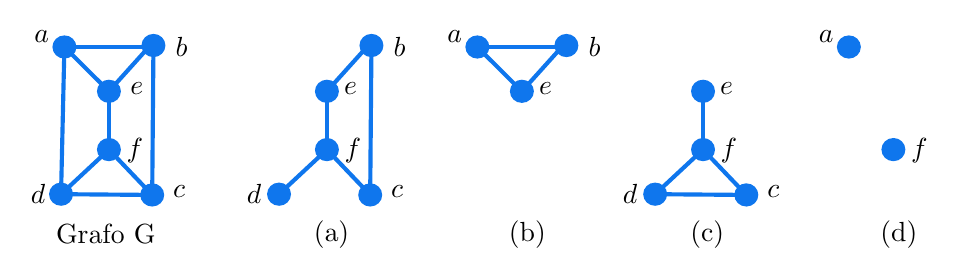
\begin{tikzpicture}[x=0.75pt,y=0.75pt,yscale=-1,xscale=1]
%uncomment if require: \path (0,138); %set diagram left start at 0, and has height of 138

%Shape: Ellipse [id:dp06213818250773073] 
\draw  [draw opacity=0][fill={rgb, 255:red, 15; green, 118; blue, 237 }  ,fill opacity=1 ] (63.6,23.59) .. controls (63.6,20.51) and (66.18,18) .. (69.37,18) .. controls (72.56,18) and (75.14,20.51) .. (75.14,23.59) .. controls (75.14,26.68) and (72.56,29.19) .. (69.37,29.19) .. controls (66.18,29.19) and (63.6,26.68) .. (63.6,23.59) -- cycle ;
%Shape: Ellipse [id:dp4065026383825223] 
\draw  [draw opacity=0][fill={rgb, 255:red, 15; green, 118; blue, 237 }  ,fill opacity=1 ] (63,95.59) .. controls (63,92.5) and (65.59,90) .. (68.77,90) .. controls (71.96,90) and (74.55,92.5) .. (74.55,95.59) .. controls (74.55,98.67) and (71.96,101.18) .. (68.77,101.18) .. controls (65.59,101.18) and (63,98.67) .. (63,95.59) -- cycle ;
%Shape: Ellipse [id:dp042507222433784575] 
\draw  [draw opacity=0][fill={rgb, 255:red, 15; green, 118; blue, 237 }  ,fill opacity=1 ] (42.15,45.66) .. controls (42.15,42.57) and (44.73,40.07) .. (47.92,40.07) .. controls (51.11,40.07) and (53.69,42.57) .. (53.69,45.66) .. controls (53.69,48.75) and (51.11,51.25) .. (47.92,51.25) .. controls (44.73,51.25) and (42.15,48.75) .. (42.15,45.66) -- cycle ;
%Shape: Ellipse [id:dp8880065091163529] 
\draw  [draw opacity=0][fill={rgb, 255:red, 15; green, 118; blue, 237 }  ,fill opacity=1 ] (19.07,95.23) .. controls (19.07,92.14) and (21.66,89.64) .. (24.85,89.64) .. controls (28.04,89.64) and (30.62,92.14) .. (30.62,95.23) .. controls (30.62,98.32) and (28.04,100.82) .. (24.85,100.82) .. controls (21.66,100.82) and (19.07,98.32) .. (19.07,95.23) -- cycle ;
%Shape: Ellipse [id:dp3510053979383396] 
\draw  [draw opacity=0][fill={rgb, 255:red, 15; green, 118; blue, 237 }  ,fill opacity=1 ] (20.7,24.31) .. controls (20.7,21.22) and (23.28,18.72) .. (26.47,18.72) .. controls (29.66,18.72) and (32.24,21.22) .. (32.24,24.31) .. controls (32.24,27.4) and (29.66,29.9) .. (26.47,29.9) .. controls (23.28,29.9) and (20.7,27.4) .. (20.7,24.31) -- cycle ;
%Straight Lines [id:da5370836499807106] 
\draw [color={rgb, 255:red, 15; green, 118; blue, 237 }  ,draw opacity=1 ][line width=1.5]    (24.85,95.23) -- (26.47,24.31) ;
%Straight Lines [id:da07197830210576894] 
\draw [color={rgb, 255:red, 15; green, 118; blue, 237 }  ,draw opacity=1 ][line width=1.5]    (67.15,24.31) -- (26.47,24.31) ;
%Straight Lines [id:da1615593071487995] 
\draw [color={rgb, 255:red, 15; green, 118; blue, 237 }  ,draw opacity=1 ][line width=1.5]    (47.92,73.74) -- (24.85,95.23) ;
%Straight Lines [id:da30907898589982774] 
\draw [color={rgb, 255:red, 15; green, 118; blue, 237 }  ,draw opacity=1 ][line width=1.5]    (68.77,95.59) -- (69.37,23.59) ;
%Straight Lines [id:da12409346993190895] 
\draw [color={rgb, 255:red, 15; green, 118; blue, 237 }  ,draw opacity=1 ][line width=1.5]    (26.47,24.31) -- (47.92,45.66) ;
%Straight Lines [id:da8093823939141009] 
\draw [color={rgb, 255:red, 15; green, 118; blue, 237 }  ,draw opacity=1 ][line width=1.5]    (67.15,24.31) -- (47.92,45.66) ;
%Shape: Ellipse [id:dp2216403453119833] 
\draw  [draw opacity=0][fill={rgb, 255:red, 15; green, 118; blue, 237 }  ,fill opacity=1 ] (42.15,73.74) .. controls (42.15,70.65) and (44.73,68.15) .. (47.92,68.15) .. controls (51.11,68.15) and (53.69,70.65) .. (53.69,73.74) .. controls (53.69,76.83) and (51.11,79.33) .. (47.92,79.33) .. controls (44.73,79.33) and (42.15,76.83) .. (42.15,73.74) -- cycle ;
%Straight Lines [id:da47606064030624573] 
\draw [color={rgb, 255:red, 15; green, 118; blue, 237 }  ,draw opacity=1 ][line width=1.5]    (47.92,45.66) -- (47.92,73.74) ;
%Straight Lines [id:da2460096165808776] 
\draw [color={rgb, 255:red, 15; green, 118; blue, 237 }  ,draw opacity=1 ][line width=1.5]    (47.92,73.74) -- (68.77,95.59) ;
%Straight Lines [id:da14123966172845392] 
\draw [color={rgb, 255:red, 15; green, 118; blue, 237 }  ,draw opacity=1 ][line width=1.5]    (68.77,95.59) -- (24.85,95.23) ;
%Shape: Ellipse [id:dp8501456895730941] 
\draw  [draw opacity=0][fill={rgb, 255:red, 15; green, 118; blue, 237 }  ,fill opacity=1 ] (168.63,23.59) .. controls (168.63,20.51) and (171.21,18) .. (174.4,18) .. controls (177.59,18) and (180.17,20.51) .. (180.17,23.59) .. controls (180.17,26.68) and (177.59,29.19) .. (174.4,29.19) .. controls (171.21,29.19) and (168.63,26.68) .. (168.63,23.59) -- cycle ;
%Shape: Ellipse [id:dp4041891528935715] 
\draw  [draw opacity=0][fill={rgb, 255:red, 15; green, 118; blue, 237 }  ,fill opacity=1 ] (168.03,95.59) .. controls (168.03,92.5) and (170.61,90) .. (173.8,90) .. controls (176.99,90) and (179.58,92.5) .. (179.58,95.59) .. controls (179.58,98.67) and (176.99,101.18) .. (173.8,101.18) .. controls (170.61,101.18) and (168.03,98.67) .. (168.03,95.59) -- cycle ;
%Shape: Ellipse [id:dp039032306124791694] 
\draw  [draw opacity=0][fill={rgb, 255:red, 15; green, 118; blue, 237 }  ,fill opacity=1 ] (147.18,45.66) .. controls (147.18,42.57) and (149.76,40.07) .. (152.95,40.07) .. controls (156.14,40.07) and (158.72,42.57) .. (158.72,45.66) .. controls (158.72,48.75) and (156.14,51.25) .. (152.95,51.25) .. controls (149.76,51.25) and (147.18,48.75) .. (147.18,45.66) -- cycle ;
%Shape: Ellipse [id:dp44328095018157865] 
\draw  [draw opacity=0][fill={rgb, 255:red, 15; green, 118; blue, 237 }  ,fill opacity=1 ] (124.1,95.23) .. controls (124.1,92.14) and (126.69,89.64) .. (129.88,89.64) .. controls (133.06,89.64) and (135.65,92.14) .. (135.65,95.23) .. controls (135.65,98.32) and (133.06,100.82) .. (129.88,100.82) .. controls (126.69,100.82) and (124.1,98.32) .. (124.1,95.23) -- cycle ;
%Straight Lines [id:da9420974055203732] 
\draw [color={rgb, 255:red, 15; green, 118; blue, 237 }  ,draw opacity=1 ][line width=1.5]    (152.95,73.74) -- (129.88,95.23) ;
%Straight Lines [id:da28477194064783795] 
\draw [color={rgb, 255:red, 15; green, 118; blue, 237 }  ,draw opacity=1 ][line width=1.5]    (173.8,95.59) -- (174.4,23.59) ;
%Straight Lines [id:da5671466196907173] 
\draw [color={rgb, 255:red, 15; green, 118; blue, 237 }  ,draw opacity=1 ][line width=1.5]    (172.18,24.31) -- (152.95,45.66) ;
%Shape: Ellipse [id:dp5072304471150608] 
\draw  [draw opacity=0][fill={rgb, 255:red, 15; green, 118; blue, 237 }  ,fill opacity=1 ] (147.18,73.74) .. controls (147.18,70.65) and (149.76,68.15) .. (152.95,68.15) .. controls (156.14,68.15) and (158.72,70.65) .. (158.72,73.74) .. controls (158.72,76.83) and (156.14,79.33) .. (152.95,79.33) .. controls (149.76,79.33) and (147.18,76.83) .. (147.18,73.74) -- cycle ;
%Straight Lines [id:da6773602653086976] 
\draw [color={rgb, 255:red, 15; green, 118; blue, 237 }  ,draw opacity=1 ][line width=1.5]    (152.95,45.66) -- (152.95,73.74) ;
%Straight Lines [id:da647926632955566] 
\draw [color={rgb, 255:red, 15; green, 118; blue, 237 }  ,draw opacity=1 ][line width=1.5]    (152.95,73.74) -- (173.8,95.59) ;
%Shape: Ellipse [id:dp12309596019443325] 
\draw  [draw opacity=0][fill={rgb, 255:red, 15; green, 118; blue, 237 }  ,fill opacity=1 ] (262.56,23.59) .. controls (262.56,20.51) and (265.15,18) .. (268.33,18) .. controls (271.52,18) and (274.11,20.51) .. (274.11,23.59) .. controls (274.11,26.68) and (271.52,29.19) .. (268.33,29.19) .. controls (265.15,29.19) and (262.56,26.68) .. (262.56,23.59) -- cycle ;
%Shape: Ellipse [id:dp6776501121426091] 
\draw  [draw opacity=0][fill={rgb, 255:red, 15; green, 118; blue, 237 }  ,fill opacity=1 ] (241.11,45.66) .. controls (241.11,42.57) and (243.7,40.07) .. (246.88,40.07) .. controls (250.07,40.07) and (252.66,42.57) .. (252.66,45.66) .. controls (252.66,48.75) and (250.07,51.25) .. (246.88,51.25) .. controls (243.7,51.25) and (241.11,48.75) .. (241.11,45.66) -- cycle ;
%Shape: Ellipse [id:dp4415792388227735] 
\draw  [draw opacity=0][fill={rgb, 255:red, 15; green, 118; blue, 237 }  ,fill opacity=1 ] (219.66,24.31) .. controls (219.66,21.22) and (222.25,18.72) .. (225.43,18.72) .. controls (228.62,18.72) and (231.21,21.22) .. (231.21,24.31) .. controls (231.21,27.4) and (228.62,29.9) .. (225.43,29.9) .. controls (222.25,29.9) and (219.66,27.4) .. (219.66,24.31) -- cycle ;
%Straight Lines [id:da758538061398145] 
\draw [color={rgb, 255:red, 15; green, 118; blue, 237 }  ,draw opacity=1 ][line width=1.5]    (266.11,24.31) -- (225.43,24.31) ;
%Straight Lines [id:da7335656275787226] 
\draw [color={rgb, 255:red, 15; green, 118; blue, 237 }  ,draw opacity=1 ][line width=1.5]    (225.43,24.31) -- (246.88,45.66) ;
%Straight Lines [id:da20594191662926908] 
\draw [color={rgb, 255:red, 15; green, 118; blue, 237 }  ,draw opacity=1 ][line width=1.5]    (266.11,24.31) -- (246.88,45.66) ;
%Shape: Ellipse [id:dp6881101772450808] 
\draw  [draw opacity=0][fill={rgb, 255:red, 15; green, 118; blue, 237 }  ,fill opacity=1 ] (349.24,95.59) .. controls (349.24,92.5) and (351.83,90) .. (355.02,90) .. controls (358.2,90) and (360.79,92.5) .. (360.79,95.59) .. controls (360.79,98.67) and (358.2,101.18) .. (355.02,101.18) .. controls (351.83,101.18) and (349.24,98.67) .. (349.24,95.59) -- cycle ;
%Shape: Ellipse [id:dp08456402208840652] 
\draw  [draw opacity=0][fill={rgb, 255:red, 15; green, 118; blue, 237 }  ,fill opacity=1 ] (328.39,45.66) .. controls (328.39,42.57) and (330.97,40.07) .. (334.16,40.07) .. controls (337.35,40.07) and (339.93,42.57) .. (339.93,45.66) .. controls (339.93,48.75) and (337.35,51.25) .. (334.16,51.25) .. controls (330.97,51.25) and (328.39,48.75) .. (328.39,45.66) -- cycle ;
%Shape: Ellipse [id:dp9279561378295653] 
\draw  [draw opacity=0][fill={rgb, 255:red, 15; green, 118; blue, 237 }  ,fill opacity=1 ] (305.32,95.23) .. controls (305.32,92.14) and (307.9,89.64) .. (311.09,89.64) .. controls (314.28,89.64) and (316.86,92.14) .. (316.86,95.23) .. controls (316.86,98.32) and (314.28,100.82) .. (311.09,100.82) .. controls (307.9,100.82) and (305.32,98.32) .. (305.32,95.23) -- cycle ;
%Straight Lines [id:da8448873943097901] 
\draw [color={rgb, 255:red, 15; green, 118; blue, 237 }  ,draw opacity=1 ][line width=1.5]    (334.16,73.74) -- (311.09,95.23) ;
%Shape: Ellipse [id:dp5836099173008862] 
\draw  [draw opacity=0][fill={rgb, 255:red, 15; green, 118; blue, 237 }  ,fill opacity=1 ] (328.39,73.74) .. controls (328.39,70.65) and (330.97,68.15) .. (334.16,68.15) .. controls (337.35,68.15) and (339.93,70.65) .. (339.93,73.74) .. controls (339.93,76.83) and (337.35,79.33) .. (334.16,79.33) .. controls (330.97,79.33) and (328.39,76.83) .. (328.39,73.74) -- cycle ;
%Straight Lines [id:da04688548949857574] 
\draw [color={rgb, 255:red, 15; green, 118; blue, 237 }  ,draw opacity=1 ][line width=1.5]    (334.16,45.66) -- (334.16,73.74) ;
%Straight Lines [id:da5912439833585417] 
\draw [color={rgb, 255:red, 15; green, 118; blue, 237 }  ,draw opacity=1 ][line width=1.5]    (334.16,73.74) -- (355.02,95.59) ;
%Straight Lines [id:da4720109759879736] 
\draw [color={rgb, 255:red, 15; green, 118; blue, 237 }  ,draw opacity=1 ][line width=1.5]    (355.02,95.59) -- (311.09,95.23) ;
%Shape: Ellipse [id:dp3898278077934265] 
\draw  [draw opacity=0][fill={rgb, 255:red, 15; green, 118; blue, 237 }  ,fill opacity=1 ] (398.65,24.31) .. controls (398.65,21.22) and (401.24,18.72) .. (404.43,18.72) .. controls (407.62,18.72) and (410.2,21.22) .. (410.2,24.31) .. controls (410.2,27.4) and (407.62,29.9) .. (404.43,29.9) .. controls (401.24,29.9) and (398.65,27.4) .. (398.65,24.31) -- cycle ;
%Shape: Ellipse [id:dp5416544246665718] 
\draw  [draw opacity=0][fill={rgb, 255:red, 15; green, 118; blue, 237 }  ,fill opacity=1 ] (420.1,73.74) .. controls (420.1,70.65) and (422.69,68.15) .. (425.88,68.15) .. controls (429.07,68.15) and (431.65,70.65) .. (431.65,73.74) .. controls (431.65,76.83) and (429.07,79.33) .. (425.88,79.33) .. controls (422.69,79.33) and (420.1,76.83) .. (420.1,73.74) -- cycle ;

% Text Node
\draw (21.17,108.29) node [anchor=north west][inner sep=0.75pt]   [align=left] {Grafo G};
% Text Node
\draw (10.78,15.27) node [anchor=north west][inner sep=0.75pt]    {$a$};
% Text Node
\draw (78.83,18.13) node [anchor=north west][inner sep=0.75pt]    {$b$};
% Text Node
\draw (77.61,89.77) node [anchor=north west][inner sep=0.75pt]    {$c$};
% Text Node
\draw (9.04,89.05) node [anchor=north west][inner sep=0.75pt]    {$d$};
% Text Node
\draw (56.94,40.34) node [anchor=north west][inner sep=0.75pt]    {$e$};
% Text Node
\draw (55.16,66.85) node [anchor=north west][inner sep=0.75pt]    {$f$};
% Text Node
\draw (145.41,106.86) node [anchor=north west][inner sep=0.75pt]   [align=left] {(a)};
% Text Node
\draw (183.86,18.13) node [anchor=north west][inner sep=0.75pt]    {$b$};
% Text Node
\draw (182.64,89.77) node [anchor=north west][inner sep=0.75pt]    {$c$};
% Text Node
\draw (113.07,89.05) node [anchor=north west][inner sep=0.75pt]    {$d$};
% Text Node
\draw (159.97,40.34) node [anchor=north west][inner sep=0.75pt]    {$e$};
% Text Node
\draw (160.19,66.85) node [anchor=north west][inner sep=0.75pt]    {$f$};
% Text Node
\draw (239.35,106.86) node [anchor=north west][inner sep=0.75pt]   [align=left] {(b)};
% Text Node
\draw (209.74,15.27) node [anchor=north west][inner sep=0.75pt]    {$a$};
% Text Node
\draw (277.79,18.13) node [anchor=north west][inner sep=0.75pt]    {$b$};
% Text Node
\draw (253.9,40.34) node [anchor=north west][inner sep=0.75pt]    {$e$};
% Text Node
\draw (326.76,106.86) node [anchor=north west][inner sep=0.75pt]   [align=left] {(c)};
% Text Node
\draw (363.85,89.77) node [anchor=north west][inner sep=0.75pt]    {$c$};
% Text Node
\draw (294.28,89.05) node [anchor=north west][inner sep=0.75pt]    {$d$};
% Text Node
\draw (341.18,40.34) node [anchor=north west][inner sep=0.75pt]    {$e$};
% Text Node
\draw (341.4,66.85) node [anchor=north west][inner sep=0.75pt]    {$f$};
% Text Node
\draw (418.34,106.86) node [anchor=north west][inner sep=0.75pt]   [align=left] {(d)};
% Text Node
\draw (388.74,15.27) node [anchor=north west][inner sep=0.75pt]    {$a$};
% Text Node
\draw (433.12,66.85) node [anchor=north west][inner sep=0.75pt]    {$f$};


\end{tikzpicture}\\

\end{ftst}

%=====

\begin{ftst}{Exercício}{Tipos de Grafos}

Considere o grafo $G$:
\vone
\centering


\tikzset{every picture/.style={line width=0.75pt}} %set default line width to 0.75pt        

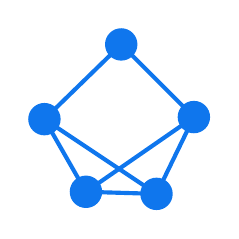
\begin{tikzpicture}[x=0.75pt,y=0.75pt,yscale=-1,xscale=1]
%uncomment if require: \path (0,113); %set diagram left start at 0, and has height of 113

%Shape: Circle [id:dp7340963082717409] 
\draw  [draw opacity=0][fill={rgb, 255:red, 15; green, 118; blue, 237 }  ,fill opacity=1 ] (44,11.81) .. controls (44,7.49) and (47.49,4) .. (51.81,4) .. controls (56.12,4) and (59.61,7.49) .. (59.61,11.81) .. controls (59.61,16.12) and (56.12,19.61) .. (51.81,19.61) .. controls (47.49,19.61) and (44,16.12) .. (44,11.81) -- cycle ;
%Shape: Circle [id:dp13193403281074279] 
\draw  [draw opacity=0][fill={rgb, 255:red, 15; green, 118; blue, 237 }  ,fill opacity=1 ] (61,83.81) .. controls (61,79.49) and (64.49,76) .. (68.81,76) .. controls (73.12,76) and (76.61,79.49) .. (76.61,83.81) .. controls (76.61,88.12) and (73.12,91.61) .. (68.81,91.61) .. controls (64.49,91.61) and (61,88.12) .. (61,83.81) -- cycle ;
%Shape: Circle [id:dp6948173250785945] 
\draw  [draw opacity=0][fill={rgb, 255:red, 15; green, 118; blue, 237 }  ,fill opacity=1 ] (79,46.81) .. controls (79,42.49) and (82.49,39) .. (86.81,39) .. controls (91.12,39) and (94.61,42.49) .. (94.61,46.81) .. controls (94.61,51.12) and (91.12,54.61) .. (86.81,54.61) .. controls (82.49,54.61) and (79,51.12) .. (79,46.81) -- cycle ;
%Shape: Circle [id:dp24106224518602137] 
\draw  [draw opacity=0][fill={rgb, 255:red, 15; green, 118; blue, 237 }  ,fill opacity=1 ] (27,82.81) .. controls (27,78.49) and (30.49,75) .. (34.81,75) .. controls (39.12,75) and (42.61,78.49) .. (42.61,82.81) .. controls (42.61,87.12) and (39.12,90.61) .. (34.81,90.61) .. controls (30.49,90.61) and (27,87.12) .. (27,82.81) -- cycle ;
%Shape: Circle [id:dp9711832352750054] 
\draw  [draw opacity=0][fill={rgb, 255:red, 15; green, 118; blue, 237 }  ,fill opacity=1 ] (7,47.81) .. controls (7,43.49) and (10.49,40) .. (14.81,40) .. controls (19.12,40) and (22.61,43.49) .. (22.61,47.81) .. controls (22.61,52.12) and (19.12,55.61) .. (14.81,55.61) .. controls (10.49,55.61) and (7,52.12) .. (7,47.81) -- cycle ;
%Straight Lines [id:da7310701003557218] 
\draw [color={rgb, 255:red, 15; green, 118; blue, 237 }  ,draw opacity=1 ][line width=1.5]    (14.81,47.81) -- (51.81,11.81) ;
%Straight Lines [id:da7752634909985894] 
\draw [color={rgb, 255:red, 15; green, 118; blue, 237 }  ,draw opacity=1 ][line width=1.5]    (86.81,46.81) -- (51.81,11.81) ;
%Straight Lines [id:da19758955378671272] 
\draw [color={rgb, 255:red, 15; green, 118; blue, 237 }  ,draw opacity=1 ][line width=1.5]    (34.81,82.81) -- (14.81,47.81) ;
%Straight Lines [id:da12430416568632707] 
\draw [color={rgb, 255:red, 15; green, 118; blue, 237 }  ,draw opacity=1 ][line width=1.5]    (68.81,83.81) -- (86.81,46.81) ;
%Straight Lines [id:da8379664401359015] 
\draw [color={rgb, 255:red, 15; green, 118; blue, 237 }  ,draw opacity=1 ][line width=1.5]    (34.81,82.81) -- (68.81,83.81) ;
%Straight Lines [id:da16929629758137388] 
\draw [color={rgb, 255:red, 15; green, 118; blue, 237 }  ,draw opacity=1 ][line width=1.5]    (34.81,82.81) -- (86.81,46.81) ;
%Straight Lines [id:da9695878442229151] 
\draw [color={rgb, 255:red, 15; green, 118; blue, 237 }  ,draw opacity=1 ][line width=1.5]    (68.81,83.81) -- (14.81,47.81) ;




\end{tikzpicture}\\
\vone
\begin{itemize}
    \item Dê nome aos seus vértices e indique o grau de cada um deles.
    \item Desenhe seu complementar $G’$.
    \item Desenhe um subgrafo simples de $G$.
    \item Desenhe um subgrafo clique de $G$.
    \item Desenhe um subgrafo induzido de $G$.
\end{itemize}

\end{ftst}


%=====

\begin{ftst}{Caminhos}{Tipos de Grafos}

Caminho de $v_1$ a $v_n$ é uma sequência de arestas $(v_1,v_2),(v_2,v_3), \dots$, $(v_{n-1}, v_n)$, denotado como: $v_1, v_2, v_3, \dots, v_{n-1}, v_n$. 
\vone
O comprimento de um caminho é o seu número de arestas.
\vone
Exemplo: caminho de $v_1$ a $v_4$ de comprimento 8.

\centering


\tikzset{every picture/.style={line width=0.75pt}} %set default line width to 0.75pt        

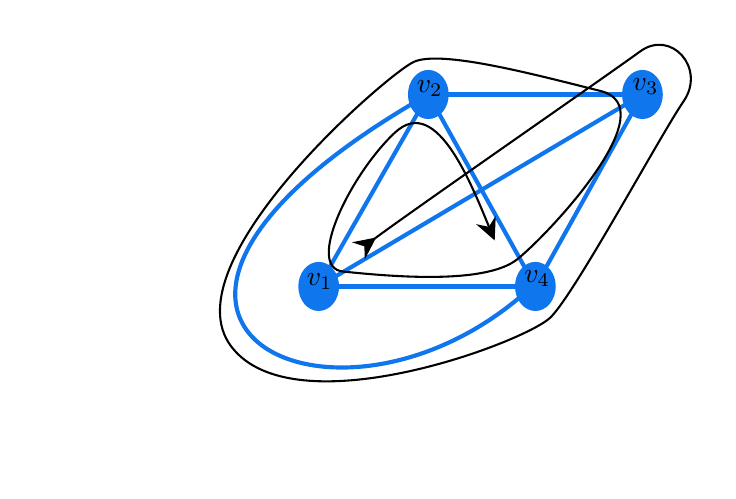
\begin{tikzpicture}[x=0.75pt,y=0.75pt,yscale=-1,xscale=1]
%uncomment if require: \path (0,191); %set diagram left start at 0, and has height of 191

%Shape: Ellipse [id:dp14942589100099868] 
\draw  [draw opacity=0][fill={rgb, 255:red, 15; green, 118; blue, 237 }  ,fill opacity=1 ] (241.97,36.83) .. controls (241.97,30.3) and (246.37,25) .. (251.79,25) .. controls (257.22,25) and (261.61,30.3) .. (261.61,36.83) .. controls (261.61,43.37) and (257.22,48.67) .. (251.79,48.67) .. controls (246.37,48.67) and (241.97,43.37) .. (241.97,36.83) -- cycle ;
%Shape: Ellipse [id:dp26449670264630165] 
\draw  [draw opacity=0][fill={rgb, 255:red, 15; green, 118; blue, 237 }  ,fill opacity=1 ] (190.4,129.32) .. controls (190.4,122.78) and (194.8,117.49) .. (200.22,117.49) .. controls (205.64,117.49) and (210.04,122.78) .. (210.04,129.32) .. controls (210.04,135.86) and (205.64,141.15) .. (200.22,141.15) .. controls (194.8,141.15) and (190.4,135.86) .. (190.4,129.32) -- cycle ;
%Shape: Ellipse [id:dp36609892365662744] 
\draw  [draw opacity=0][fill={rgb, 255:red, 15; green, 118; blue, 237 }  ,fill opacity=1 ] (86,129.32) .. controls (86,122.78) and (90.4,117.49) .. (95.82,117.49) .. controls (101.24,117.49) and (105.64,122.78) .. (105.64,129.32) .. controls (105.64,135.86) and (101.24,141.15) .. (95.82,141.15) .. controls (90.4,141.15) and (86,135.86) .. (86,129.32) -- cycle ;
%Shape: Ellipse [id:dp5281882999587482] 
\draw  [draw opacity=0][fill={rgb, 255:red, 15; green, 118; blue, 237 }  ,fill opacity=1 ] (138.83,36.83) .. controls (138.83,30.3) and (143.23,25) .. (148.65,25) .. controls (154.07,25) and (158.47,30.3) .. (158.47,36.83) .. controls (158.47,43.37) and (154.07,48.67) .. (148.65,48.67) .. controls (143.23,48.67) and (138.83,43.37) .. (138.83,36.83) -- cycle ;
%Straight Lines [id:da08080292503059483] 
\draw [color={rgb, 255:red, 15; green, 118; blue, 237 }  ,draw opacity=1 ][line width=1.5]    (200.22,129.32) -- (95.82,129.32) ;
%Straight Lines [id:da1787964975304872] 
\draw [color={rgb, 255:red, 15; green, 118; blue, 237 }  ,draw opacity=1 ][line width=1.5]    (200.22,129.32) -- (148.65,36.83) ;
%Straight Lines [id:da8679202680250606] 
\draw [color={rgb, 255:red, 15; green, 118; blue, 237 }  ,draw opacity=1 ][line width=1.5]    (200.22,129.32) -- (251.79,36.83) ;
%Straight Lines [id:da9998937901344604] 
\draw [color={rgb, 255:red, 15; green, 118; blue, 237 }  ,draw opacity=1 ][line width=1.5]    (95.82,129.32) -- (251.79,36.83) ;
%Straight Lines [id:da09608569429847669] 
\draw [color={rgb, 255:red, 15; green, 118; blue, 237 }  ,draw opacity=1 ][line width=1.5]    (95.82,129.32) -- (148.65,36.83) ;
%Straight Lines [id:da7021655238376456] 
\draw [color={rgb, 255:red, 15; green, 118; blue, 237 }  ,draw opacity=1 ][line width=1.5]    (251.79,36.83) -- (148.65,36.83) ;
%Curve Lines [id:da38006553727085524] 
\draw [line width=0.75]    (122.54,106.46) .. controls (143.51,90.9) and (235.84,26.98) .. (250.61,16.15) .. controls (265.61,5.15) and (282.61,24.15) .. (271.61,40.15) .. controls (260.61,56.15) and (219.61,132.15) .. (207.61,144.15) .. controls (195.61,156.15) and (83.61,198.15) .. (53.61,158.15) .. controls (23.61,118.15) and (128.61,27.15) .. (141.61,21.15) .. controls (154.61,15.15) and (199.61,27.15) .. (231.61,35.15) .. controls (263.61,43.15) and (207.61,103.15) .. (191.61,116.15) .. controls (175.61,129.15) and (126.13,124.02) .. (107.61,122.15) .. controls (89.09,120.28) and (111.22,75.13) .. (132.61,55.15) .. controls (153.14,35.97) and (170.2,82.19) .. (179.49,104.5) ;
\draw [shift={(180.61,107.15)}, rotate = 246.8] [fill={rgb, 255:red, 0; green, 0; blue, 0 }  ][line width=0.08]  [draw opacity=0] (10.72,-5.15) -- (0,0) -- (10.72,5.15) -- (7.12,0) -- cycle    ;
\draw [shift={(123.52,105.74)}, rotate = 503.13] [fill={rgb, 255:red, 0; green, 0; blue, 0 }  ][line width=0.08]  [draw opacity=0] (10.72,-5.15) -- (0,0) -- (10.72,5.15) -- (7.12,0) -- cycle    ;
%Curve Lines [id:da5359394739212069] 
\draw [color={rgb, 255:red, 15; green, 118; blue, 237 }  ,draw opacity=1 ][line width=1.5]    (148.65,36.83) .. controls (-43.39,146.15) and (106.61,217.15) .. (200,128) ;

% Text Node
\draw (88.82,121.72) node [anchor=north west][inner sep=0.75pt]    {$v_{1}$};
% Text Node
\draw (141.82,28.72) node [anchor=north west][inner sep=0.75pt]    {$v_{2}$};
% Text Node
\draw (245.82,27.72) node [anchor=north west][inner sep=0.75pt]    {$v_{3}$};
% Text Node
\draw (193.61,120.55) node [anchor=north west][inner sep=0.75pt]    {$v_{4}$};


\end{tikzpicture}\\


\end{ftst}

%=====

\begin{ftst}{circuitos}{Tipos de Grafos}
É um caminho de $v_1$ a $v_n$, onde $v_1 = v_n$ e nenhuma aresta é repetida.
\vone
Ex: circuito de $v_1$ a $v_1$ de comprimento 5.

\vone
\centering


\tikzset{every picture/.style={line width=0.75pt}} %set default line width to 0.75pt        

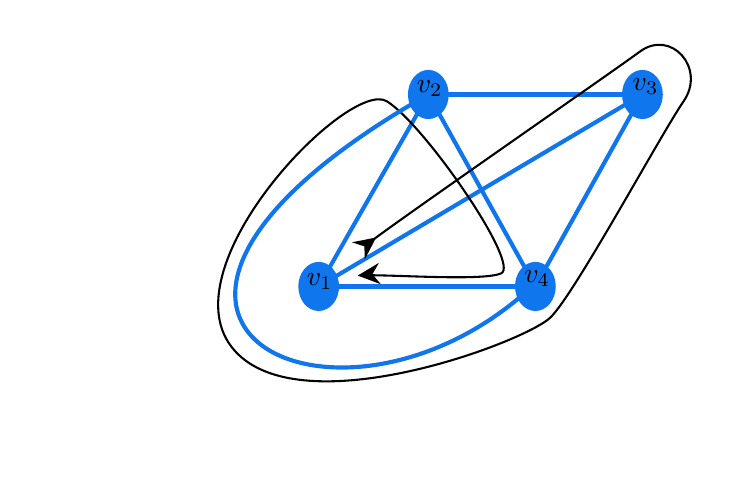
\begin{tikzpicture}[x=0.75pt,y=0.75pt,yscale=-1,xscale=1]
%uncomment if require: \path (0,193); %set diagram left start at 0, and has height of 193

%Shape: Ellipse [id:dp6446268735502532] 
\draw  [draw opacity=0][fill={rgb, 255:red, 15; green, 118; blue, 237 }  ,fill opacity=1 ] (215.97,35.83) .. controls (215.97,29.3) and (220.37,24) .. (225.79,24) .. controls (231.22,24) and (235.61,29.3) .. (235.61,35.83) .. controls (235.61,42.37) and (231.22,47.67) .. (225.79,47.67) .. controls (220.37,47.67) and (215.97,42.37) .. (215.97,35.83) -- cycle ;
%Shape: Ellipse [id:dp5426228859900855] 
\draw  [draw opacity=0][fill={rgb, 255:red, 15; green, 118; blue, 237 }  ,fill opacity=1 ] (164.4,128.32) .. controls (164.4,121.78) and (168.8,116.49) .. (174.22,116.49) .. controls (179.64,116.49) and (184.04,121.78) .. (184.04,128.32) .. controls (184.04,134.86) and (179.64,140.15) .. (174.22,140.15) .. controls (168.8,140.15) and (164.4,134.86) .. (164.4,128.32) -- cycle ;
%Shape: Ellipse [id:dp6391422210469233] 
\draw  [draw opacity=0][fill={rgb, 255:red, 15; green, 118; blue, 237 }  ,fill opacity=1 ] (60,128.32) .. controls (60,121.78) and (64.4,116.49) .. (69.82,116.49) .. controls (75.24,116.49) and (79.64,121.78) .. (79.64,128.32) .. controls (79.64,134.86) and (75.24,140.15) .. (69.82,140.15) .. controls (64.4,140.15) and (60,134.86) .. (60,128.32) -- cycle ;
%Shape: Ellipse [id:dp3528645574747755] 
\draw  [draw opacity=0][fill={rgb, 255:red, 15; green, 118; blue, 237 }  ,fill opacity=1 ] (112.83,35.83) .. controls (112.83,29.3) and (117.23,24) .. (122.65,24) .. controls (128.07,24) and (132.47,29.3) .. (132.47,35.83) .. controls (132.47,42.37) and (128.07,47.67) .. (122.65,47.67) .. controls (117.23,47.67) and (112.83,42.37) .. (112.83,35.83) -- cycle ;
%Straight Lines [id:da495082918303936] 
\draw [color={rgb, 255:red, 15; green, 118; blue, 237 }  ,draw opacity=1 ][line width=1.5]    (174.22,128.32) -- (69.82,128.32) ;
%Straight Lines [id:da5191862136160008] 
\draw [color={rgb, 255:red, 15; green, 118; blue, 237 }  ,draw opacity=1 ][line width=1.5]    (174.22,128.32) -- (122.65,35.83) ;
%Straight Lines [id:da7341802425942472] 
\draw [color={rgb, 255:red, 15; green, 118; blue, 237 }  ,draw opacity=1 ][line width=1.5]    (174.22,128.32) -- (225.79,35.83) ;
%Straight Lines [id:da34230761636576323] 
\draw [color={rgb, 255:red, 15; green, 118; blue, 237 }  ,draw opacity=1 ][line width=1.5]    (69.82,128.32) -- (225.79,35.83) ;
%Straight Lines [id:da2058619078624122] 
\draw [color={rgb, 255:red, 15; green, 118; blue, 237 }  ,draw opacity=1 ][line width=1.5]    (69.82,128.32) -- (122.65,35.83) ;
%Straight Lines [id:da9353037534202] 
\draw [color={rgb, 255:red, 15; green, 118; blue, 237 }  ,draw opacity=1 ][line width=1.5]    (225.79,35.83) -- (122.65,35.83) ;
%Curve Lines [id:da043111183117537255] 
\draw [line width=0.75]    (96.54,105.46) .. controls (117.51,89.9) and (209.84,25.98) .. (224.61,15.15) .. controls (239.61,4.15) and (256.61,23.15) .. (245.61,39.15) .. controls (234.61,55.15) and (193.61,131.15) .. (181.61,143.15) .. controls (169.61,155.15) and (57.61,197.15) .. (27.61,157.15) .. controls (-2.39,117.15) and (84.61,28.09) .. (102.61,39.09) .. controls (120.61,50.09) and (167.61,118.09) .. (157.61,122.09) .. controls (148.31,125.81) and (106.14,122.61) .. (91.44,122.95) ;
\draw [shift={(88.61,123.09)}, rotate = 354.81] [fill={rgb, 255:red, 0; green, 0; blue, 0 }  ][line width=0.08]  [draw opacity=0] (10.72,-5.15) -- (0,0) -- (10.72,5.15) -- (7.12,0) -- cycle    ;
\draw [shift={(97.52,104.74)}, rotate = 503.13] [fill={rgb, 255:red, 0; green, 0; blue, 0 }  ][line width=0.08]  [draw opacity=0] (10.72,-5.15) -- (0,0) -- (10.72,5.15) -- (7.12,0) -- cycle    ;
%Curve Lines [id:da5453842207343367] 
\draw [color={rgb, 255:red, 15; green, 118; blue, 237 }  ,draw opacity=1 ][line width=1.5]    (122.65,35.83) .. controls (-69.39,145.15) and (80.61,216.15) .. (174,127) ;

% Text Node
\draw (62.82,120.72) node [anchor=north west][inner sep=0.75pt]    {$v_{1}$};
% Text Node
\draw (115.82,27.72) node [anchor=north west][inner sep=0.75pt]    {$v_{2}$};
% Text Node
\draw (219.82,26.72) node [anchor=north west][inner sep=0.75pt]    {$v_{3}$};
% Text Node
\draw (167.61,119.55) node [anchor=north west][inner sep=0.75pt]    {$v_{4}$};


\end{tikzpicture}\\


\end{ftst}

%=====

\begin{ftst}{Ciclo}{Tipos de Grafos}
É um circuito onde nenhum vértice é repetido.
\vone
Um laço é um ciclo de comprimento 1.
\vone
Ex: ciclo de $v_1$ a $v_1$ de comprimento 4.

\vone
\centering


\tikzset{every picture/.style={line width=0.75pt}} %set default line width to 0.75pt        

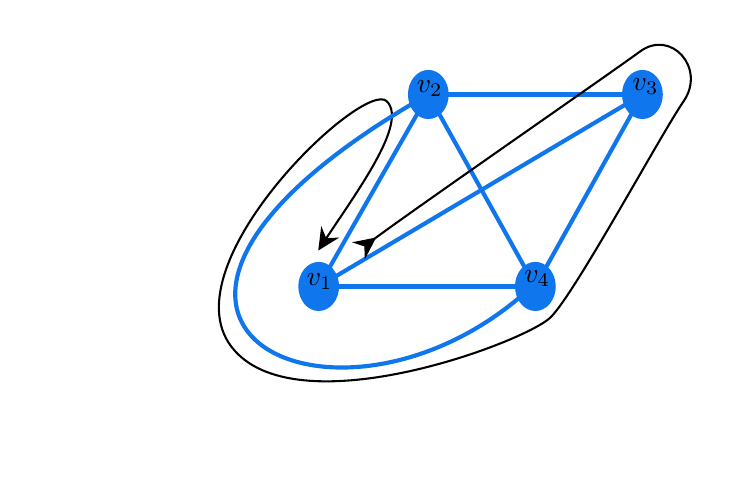
\begin{tikzpicture}[x=0.75pt,y=0.75pt,yscale=-1,xscale=1]
%uncomment if require: \path (0,191); %set diagram left start at 0, and has height of 191

%Shape: Ellipse [id:dp34898321558853973] 
\draw  [draw opacity=0][fill={rgb, 255:red, 15; green, 118; blue, 237 }  ,fill opacity=1 ] (216.97,34.83) .. controls (216.97,28.3) and (221.37,23) .. (226.79,23) .. controls (232.22,23) and (236.61,28.3) .. (236.61,34.83) .. controls (236.61,41.37) and (232.22,46.67) .. (226.79,46.67) .. controls (221.37,46.67) and (216.97,41.37) .. (216.97,34.83) -- cycle ;
%Shape: Ellipse [id:dp8581997419007412] 
\draw  [draw opacity=0][fill={rgb, 255:red, 15; green, 118; blue, 237 }  ,fill opacity=1 ] (165.4,127.32) .. controls (165.4,120.78) and (169.8,115.49) .. (175.22,115.49) .. controls (180.64,115.49) and (185.04,120.78) .. (185.04,127.32) .. controls (185.04,133.86) and (180.64,139.15) .. (175.22,139.15) .. controls (169.8,139.15) and (165.4,133.86) .. (165.4,127.32) -- cycle ;
%Shape: Ellipse [id:dp41884719294805106] 
\draw  [draw opacity=0][fill={rgb, 255:red, 15; green, 118; blue, 237 }  ,fill opacity=1 ] (61,127.32) .. controls (61,120.78) and (65.4,115.49) .. (70.82,115.49) .. controls (76.24,115.49) and (80.64,120.78) .. (80.64,127.32) .. controls (80.64,133.86) and (76.24,139.15) .. (70.82,139.15) .. controls (65.4,139.15) and (61,133.86) .. (61,127.32) -- cycle ;
%Shape: Ellipse [id:dp30805206221575077] 
\draw  [draw opacity=0][fill={rgb, 255:red, 15; green, 118; blue, 237 }  ,fill opacity=1 ] (113.83,34.83) .. controls (113.83,28.3) and (118.23,23) .. (123.65,23) .. controls (129.07,23) and (133.47,28.3) .. (133.47,34.83) .. controls (133.47,41.37) and (129.07,46.67) .. (123.65,46.67) .. controls (118.23,46.67) and (113.83,41.37) .. (113.83,34.83) -- cycle ;
%Straight Lines [id:da3826380092967572] 
\draw [color={rgb, 255:red, 15; green, 118; blue, 237 }  ,draw opacity=1 ][line width=1.5]    (175.22,127.32) -- (70.82,127.32) ;
%Straight Lines [id:da4106819955823968] 
\draw [color={rgb, 255:red, 15; green, 118; blue, 237 }  ,draw opacity=1 ][line width=1.5]    (175.22,127.32) -- (123.65,34.83) ;
%Straight Lines [id:da7580501785731988] 
\draw [color={rgb, 255:red, 15; green, 118; blue, 237 }  ,draw opacity=1 ][line width=1.5]    (175.22,127.32) -- (226.79,34.83) ;
%Straight Lines [id:da969517746532589] 
\draw [color={rgb, 255:red, 15; green, 118; blue, 237 }  ,draw opacity=1 ][line width=1.5]    (70.82,127.32) -- (226.79,34.83) ;
%Straight Lines [id:da6582184521191663] 
\draw [color={rgb, 255:red, 15; green, 118; blue, 237 }  ,draw opacity=1 ][line width=1.5]    (70.82,127.32) -- (123.65,34.83) ;
%Straight Lines [id:da21183924681168675] 
\draw [color={rgb, 255:red, 15; green, 118; blue, 237 }  ,draw opacity=1 ][line width=1.5]    (226.79,34.83) -- (123.65,34.83) ;
%Curve Lines [id:da3222564220290218] 
\draw [line width=0.75]    (97.54,104.46) .. controls (118.51,88.9) and (210.84,24.98) .. (225.61,14.15) .. controls (240.61,3.15) and (257.61,22.15) .. (246.61,38.15) .. controls (235.61,54.15) and (194.61,130.15) .. (182.61,142.15) .. controls (170.61,154.15) and (58.61,196.15) .. (28.61,156.15) .. controls (-1.39,116.15) and (92.61,27.16) .. (103.61,38.09) .. controls (114.28,48.7) and (88.26,82.89) .. (72.08,107.75) ;
\draw [shift={(70.61,110.03)}, rotate = 302.62] [fill={rgb, 255:red, 0; green, 0; blue, 0 }  ][line width=0.08]  [draw opacity=0] (10.72,-5.15) -- (0,0) -- (10.72,5.15) -- (7.12,0) -- cycle    ;
\draw [shift={(98.52,103.74)}, rotate = 503.13] [fill={rgb, 255:red, 0; green, 0; blue, 0 }  ][line width=0.08]  [draw opacity=0] (10.72,-5.15) -- (0,0) -- (10.72,5.15) -- (7.12,0) -- cycle    ;
%Curve Lines [id:da7766481202964295] 
\draw [color={rgb, 255:red, 15; green, 118; blue, 237 }  ,draw opacity=1 ][line width=1.5]    (123.65,34.83) .. controls (-68.39,144.15) and (81.61,215.15) .. (175,126) ;

% Text Node
\draw (63.82,119.72) node [anchor=north west][inner sep=0.75pt]    {$v_{1}$};
% Text Node
\draw (116.82,26.72) node [anchor=north west][inner sep=0.75pt]    {$v_{2}$};
% Text Node
\draw (220.82,25.72) node [anchor=north west][inner sep=0.75pt]    {$v_{3}$};
% Text Node
\draw (168.61,118.55) node [anchor=north west][inner sep=0.75pt]    {$v_{4}$};


\end{tikzpicture}\\


\end{ftst}

%=====

\begin{ftst}{Grau de um Vértice}{Teoria dos grafos}
\justifying
O grau de um vértice é definido como o número de arestas incidentes em tal vértice.
\vone
\vone
\centering


\tikzset{every picture/.style={line width=0.75pt}} %set default line width to 0.75pt        

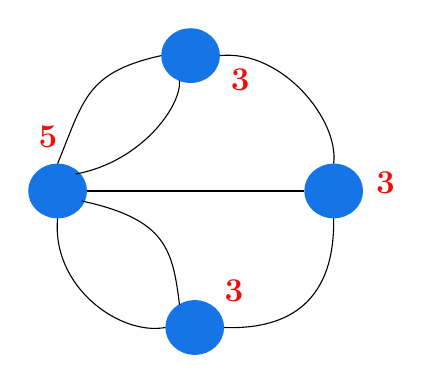
\begin{tikzpicture}[x=0.75pt,y=0.75pt,yscale=-1,xscale=1]
%uncomment if require: \path (0,177); %set diagram left start at 0, and has height of 177

%Shape: Ellipse [id:dp8878451264053866] 
\draw  [draw opacity=0][fill={rgb, 255:red, 21; green, 117; blue, 231 }  ,fill opacity=1 ] (68.33,18.19) .. controls (68.33,10.9) and (74.66,5) .. (82.48,5) .. controls (90.29,5) and (96.63,10.9) .. (96.63,18.19) .. controls (96.63,25.47) and (90.29,31.37) .. (82.48,31.37) .. controls (74.66,31.37) and (68.33,25.47) .. (68.33,18.19) -- cycle ;
%Shape: Ellipse [id:dp2916294149093952] 
\draw  [draw opacity=0][fill={rgb, 255:red, 21; green, 117; blue, 231 }  ,fill opacity=1 ] (137.27,83.42) .. controls (137.27,76.13) and (143.61,70.23) .. (151.42,70.23) .. controls (159.24,70.23) and (165.58,76.13) .. (165.58,83.42) .. controls (165.58,90.7) and (159.24,96.6) .. (151.42,96.6) .. controls (143.61,96.6) and (137.27,90.7) .. (137.27,83.42) -- cycle ;
%Shape: Ellipse [id:dp3230435826467881] 
\draw  [draw opacity=0][fill={rgb, 255:red, 21; green, 117; blue, 231 }  ,fill opacity=1 ] (70.33,149.19) .. controls (70.33,141.9) and (76.66,136) .. (84.48,136) .. controls (92.29,136) and (98.63,141.9) .. (98.63,149.19) .. controls (98.63,156.47) and (92.29,162.37) .. (84.48,162.37) .. controls (76.66,162.37) and (70.33,156.47) .. (70.33,149.19) -- cycle ;
%Shape: Ellipse [id:dp43124705110127093] 
\draw  [draw opacity=0][fill={rgb, 255:red, 21; green, 117; blue, 231 }  ,fill opacity=1 ] (4.27,83.42) .. controls (4.27,76.13) and (10.61,70.23) .. (18.42,70.23) .. controls (26.24,70.23) and (32.58,76.13) .. (32.58,83.42) .. controls (32.58,90.7) and (26.24,96.6) .. (18.42,96.6) .. controls (10.61,96.6) and (4.27,90.7) .. (4.27,83.42) -- cycle ;
%Curve Lines [id:da2175749921862662] 
\draw    (18.42,70.23) .. controls (31.15,39.25) and (32.15,26.25) .. (68.33,18.19) ;
%Curve Lines [id:da3475393637016071] 
\draw    (70.33,149.19) .. controls (48.33,153.19) and (15.42,129.6) .. (18.42,96.6) ;
%Curve Lines [id:da8464775768749004] 
\draw    (77.15,138.25) .. controls (73.83,111.49) and (70.73,97.08) .. (30.15,88.25) ;
%Curve Lines [id:da2560797041651943] 
\draw    (27.15,75.25) .. controls (59.15,69.25) and (78.15,42.25) .. (77.15,30.25) ;
%Curve Lines [id:da7980507121214329] 
\draw    (151.42,70.23) .. controls (154.15,49.25) and (126.63,15.19) .. (96.63,18.19) ;
%Curve Lines [id:da8344460663280768] 
\draw    (151.42,96.6) .. controls (152.15,140.25) and (125.63,150.19) .. (98.63,149.19) ;
%Straight Lines [id:da00593623081886796] 
\draw    (32.58,83.42) -- (137.27,83.42) ;

% Text Node
\draw (8,51) node [anchor=north west][inner sep=0.75pt]  [font=\large] [align=left] {\textbf{\textcolor[rgb]{0.95,0.05,0.05}{5}}};
% Text Node
\draw (100.63,23.19) node [anchor=north west][inner sep=0.75pt]  [font=\large] [align=left] {\textbf{\textcolor[rgb]{0.95,0.05,0.05}{3}}};
% Text Node
\draw (170.63,73.19) node [anchor=north west][inner sep=0.75pt]  [font=\large] [align=left] {\textbf{\textcolor[rgb]{0.95,0.05,0.05}{3}}};
% Text Node
\draw (97.63,125.19) node [anchor=north west][inner sep=0.75pt]  [font=\large] [align=left] {\textbf{\textcolor[rgb]{0.95,0.05,0.05}{3}}};


\end{tikzpicture}\\


\end{ftst}

%=====

\begin{ftst}{Exercício}{Teoria dos grafos}
\justifying
\textbf{Teorema 1}: a soma dos graus de todos os vértices de um grafo G é igual a duas vezes o número de arestas do grafo.
\vone
\textbf{Teorema 2}: o número de vértices de grau ímpar de um grafo é sempre par.
\vone
\textbf{Pergunta}: Se G é um grafo com 14 vértices e 25 arestas, cujos vértices têm grau 3 ou 5, quantos vértices tem grau 3 e quantos tem grau 5?



\end{ftst}

%=====



\end{document}